\everymath{\displaystyle}
\documentclass{beamer}
% \documentclass[handout]{beamer}

%\usepackage[pdftex]{color,graphicx}
\usepackage{amsmath,amssymb,amsfonts}

\mode<presentation>
{
  % \usetheme{Darmstadt}
  % \usetheme[hideothersubsections]{Hannover}
  % \usetheme[hideothersubsections]{Goettingen}
  \usetheme[hideothersubsections, right]{Berkeley}

  \usecolortheme{seahorse}
  % \usecolortheme{dolphin}
  \usecolortheme{rose}
  % \usecolortheme{orchid}

  \useinnertheme[shadow]{rounded}

  % \setbeamercovered{transparent}
  \setbeamercovered{invisible}
  % or whatever (possibly just delete it)
}

\mode<handout>{
  \setbeamercolor{background canvas}{bg=black!5}
  \usepackage{pgfpages}
  \pgfpagesuselayout{4 on 1}[a4paper,border shrink=5mm, landscape]
}

\usepackage[brazilian]{babel}
% or whatever

% \usepackage[latin1]{inputenc}
\usepackage[utf8]{inputenc}
% or whatever

\usepackage{times}
%\usepackage[T1]{fontenc}
% Or whatever. Note that the encoding and the font should match. If T1
% does not look nice, try deleting the line with the fontenc.


\title%[] % (optional, use only with long paper titles)
{Comparações múltiplas e ANOVA}

\subtitle
{Teste paramétrico para 3 ou mais grupos (quantitativo)} % (optional)

\author%[] % (optional, use only with lots of authors)
{Felipe Figueiredo}% \and S.~Another\inst{2}}
% - Use the \inst{?} command only if the authors have different
%   affiliation.

\institute[INTO] % (optional, but mostly needed)
{Instituto Nacional de Traumatologia e Ortopedia
}
  % \inst{1}%
  % Department of Computer Science\\
  % University of Somewhere
  % \and
  % \inst{2}%
  % Department of Theoretical Philosophy\\
  % University of Elsewhere}
% - Use the \inst command only if there are several affiliations.
% - Keep it simple, no one is interested in your street address.

\date%[] % (optional)
{}

% \subject{Talks}
% This is only inserted into the PDF information catalog. Can be left
% out. 



% If you have a file called "university-logo-filename.xxx", where xxx
% is a graphic format that can be processed by latex or pdflatex,
% resp., then you can add a logo as follows:

\pgfdeclareimage[height=1.6cm]{university-logo}{../logo}
\logo{\pgfuseimage{university-logo}}



% Delete this, if you do not want the table of contents to pop up at
% the beginning of each subsection:
\AtBeginSubsection[]
%\AtBeginSection[]
{
  \begin{frame}<beamer>{Sumário}
    \tableofcontents[currentsection,currentsubsection]
  \end{frame}
}


% If you wish to uncover everything in a step-wise fashion, uncomment
% the following command: 

% \beamerdefaultoverlayspecification{<+->}

\usepackage[normalem]{ulem}

\begin{document}

\begin{frame}
  \titlepage
\end{frame}

\begin{frame}{Sumário}
  \tableofcontents
  % You might wish to add the option [pausesections]
\end{frame}


%% Template
% \section{}

% \subsection{}

% \begin{frame}{}
%   \begin{itemize}
%   \item 
%   \end{itemize}
% \end{frame}

% \begin{frame}
%   \begin{columns}
%     \begin{column}{5cm}
%     \end{column}
%     \begin{column}{5cm}
%     \end{column}
%   \end{columns}
% \end{frame}

% \begin{frame}{}
%   \includegraphics[height=0.4\textheight]{file1}
%   \includegraphics[height=0.4\textheight]{file2}
%   \includegraphics[height=0.4\textheight]{file3}
%   \begin{figure}
%     \caption{}
%   \end{figure}
% \end{frame}

% \begin{frame}{}
%   \begin{definition}
%   \end{definition}
%   \begin{example}
%   \end{example}
%   \begin{block}{Exercício}
%   \end{block}
% \end{frame}

\section{Discussão da aula passada}

\subsection{Discussão da aula passada}

\begin{frame}{Discussão da aula passada}
  \begin{block}{}
    Discussão da leitura obrigatória da aula passada
  \end{block}
\end{frame}

\section{Comparações múltiplas}

\subsection{Comparações múltiplas}

\begin{frame}{Como comparar três ou mais grupos?}
  \begin{itemize}
  \item ``Comparar'' é um termo vago - precisamos de um critério bem definido!
  \end{itemize}
  \begin{block}{Para comparar quanto às variâncias dos grupos}
    Podemos usar
    \begin{itemize}
    \item Teste de Levene
    \item Teste de Bartlett
    \end{itemize}
  \end{block}
  \begin{block}{Para comparar quanto às médias dos grupos}
    {\em Pay attention}
  \end{block}
\end{frame}
  
\begin{frame}[label=requisito]{Como comparar médias}
  \begin{itemize}
  \item Vimos que o {\bf teste t} pode ser usado para comparar duas médias
  \item Assumindo que atendemos às premissas do teste t, precisamos levar em conta:
    \begin{itemize}
    \item variabilidade dos grupos
    \item tamanho do estudo (n)
    \end{itemize}
  \end{itemize}
  \begin{block}{Requisitos não óbvios (além das médias)}
    desvio padrão + n = erro padrão
  \end{block}
\end{frame}

\begin{frame}
  \begin{block}{}
    O que é necessário para decidir se 3 (ou mais) grupos possuem médias diferentes?
  \end{block}
\end{frame}

\begin{frame}[label=cenario1]{\small Cenário 1 -- esses 3 grupos têm médias diferentes?}
  \begin{center}
    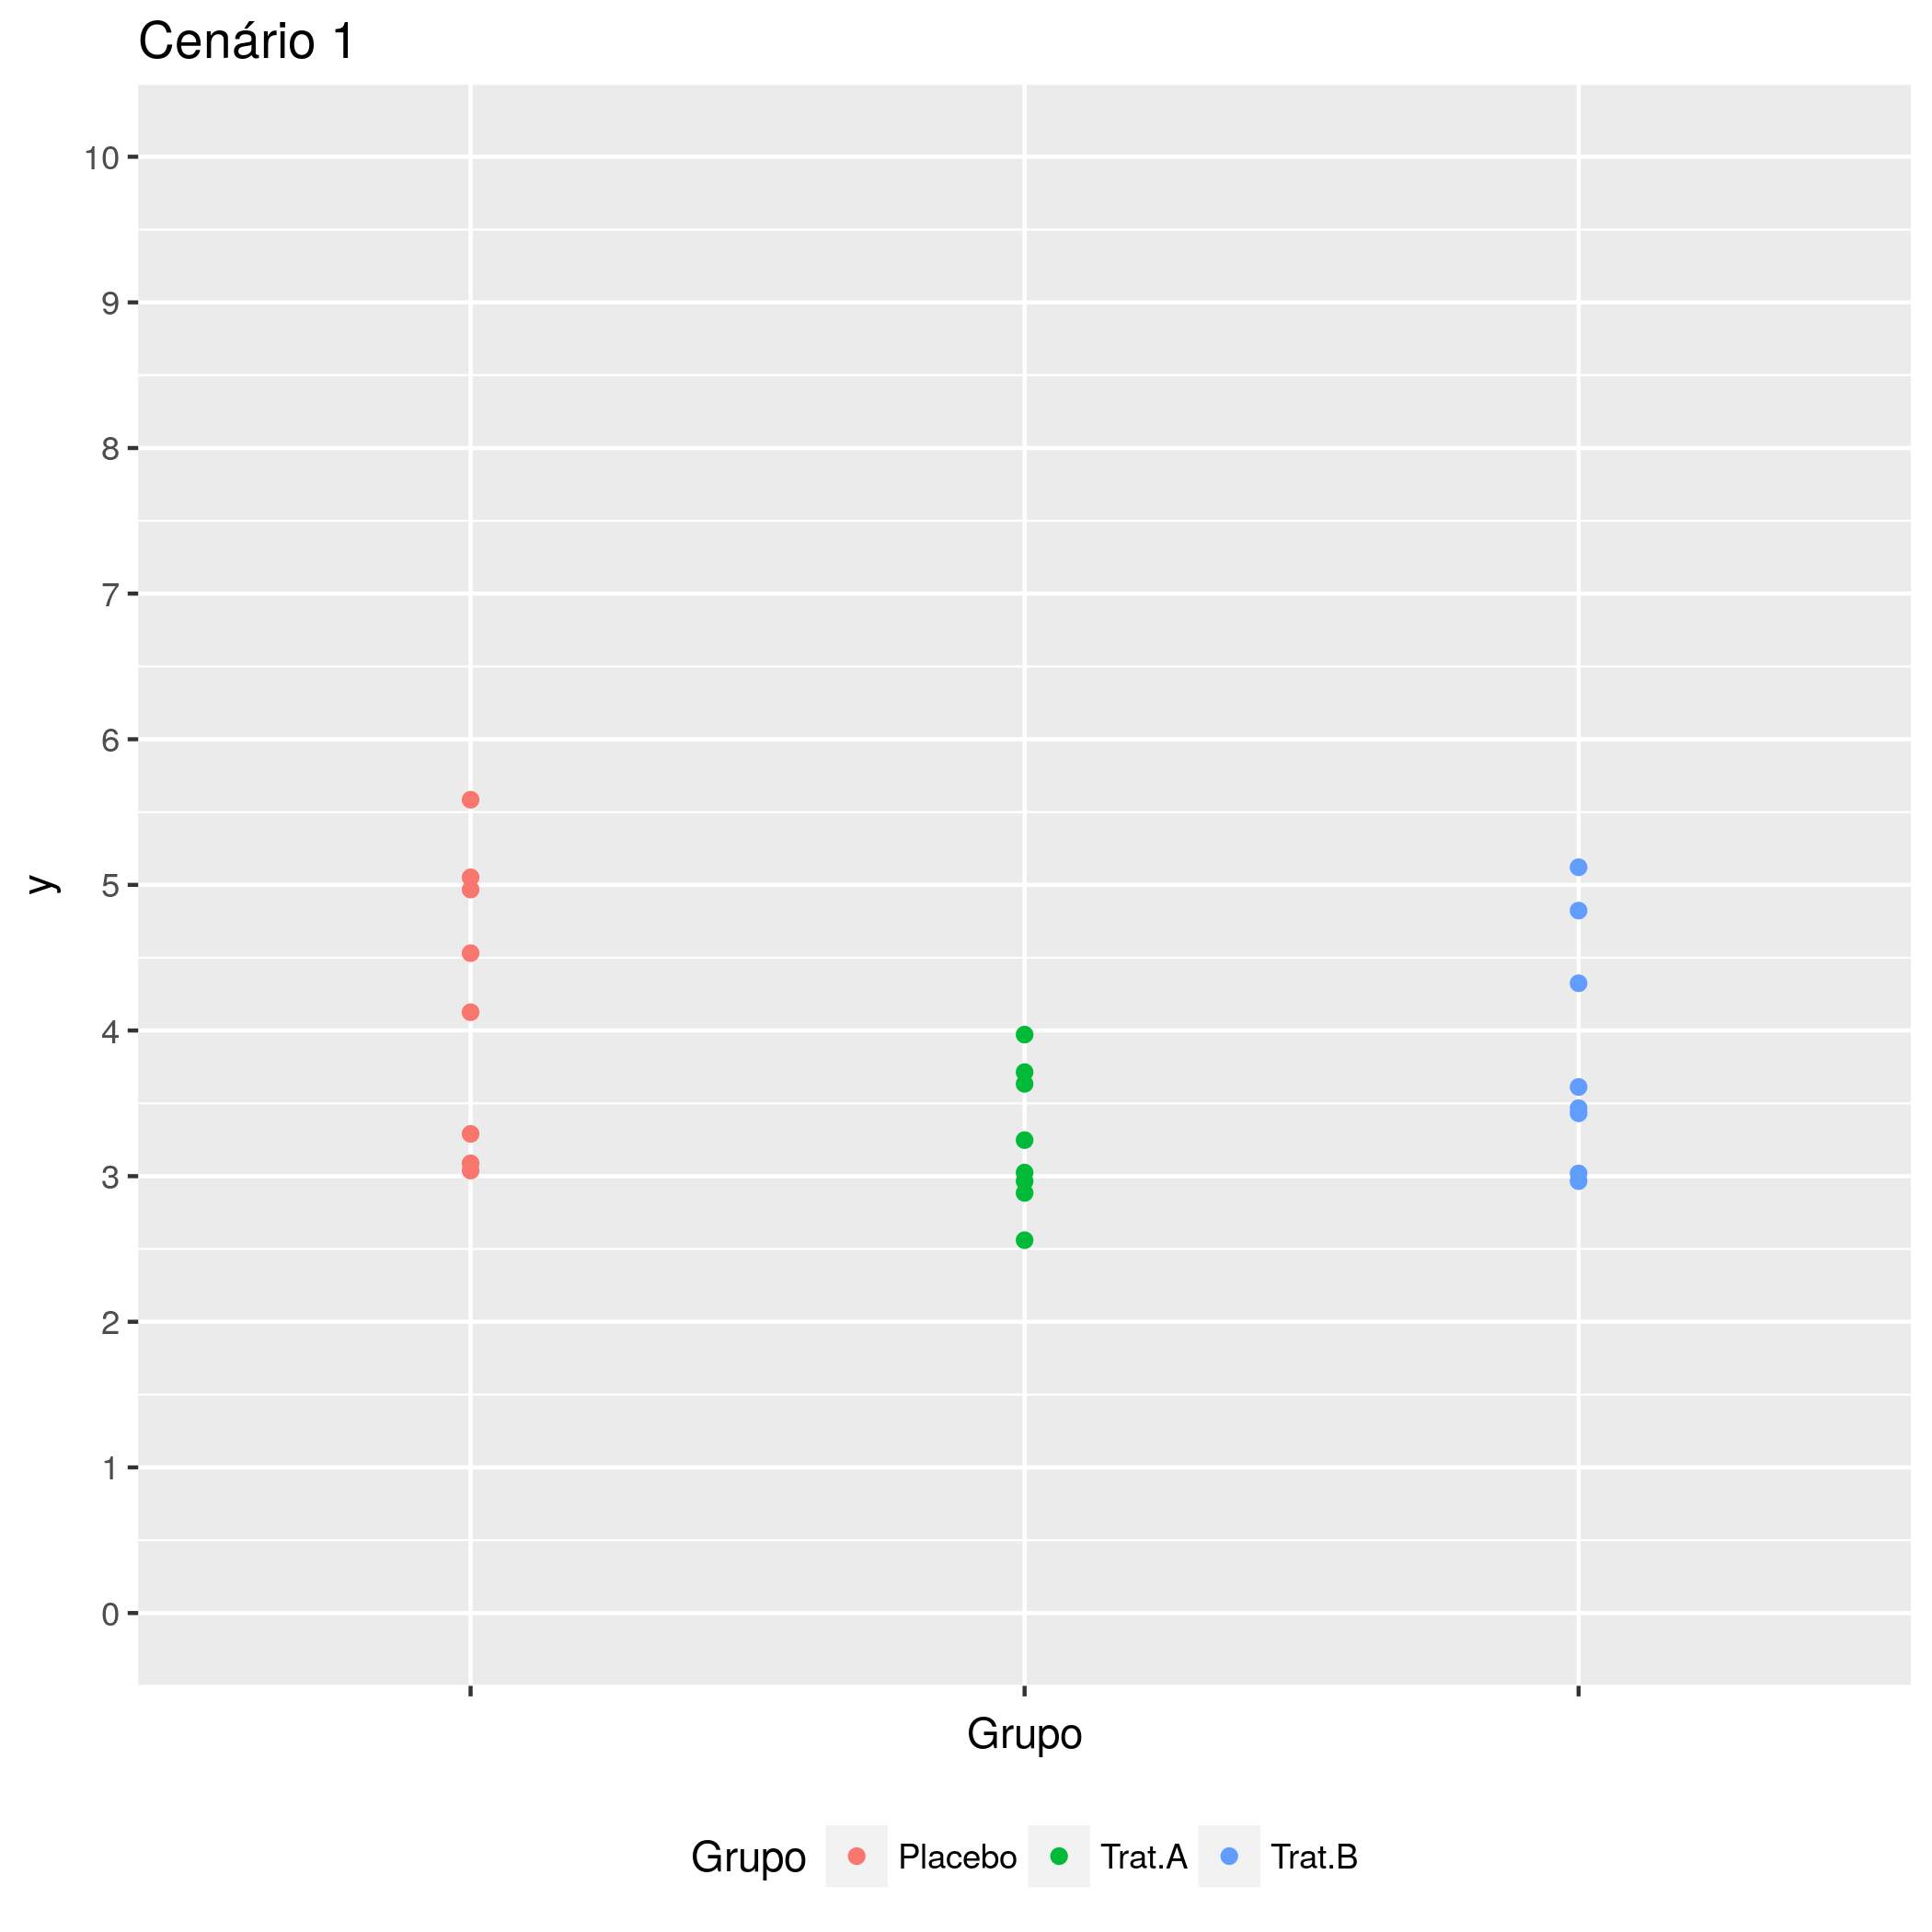
\includegraphics[height=.9\textheight]{Cap13-30/cenario1}
  \end{center}
\end{frame}

\begin{frame}{\footnotesize Médias: Placebo: 5.945, Tratamento A: 5.027, Tratamento B: 5.110}
  \begin{center}
    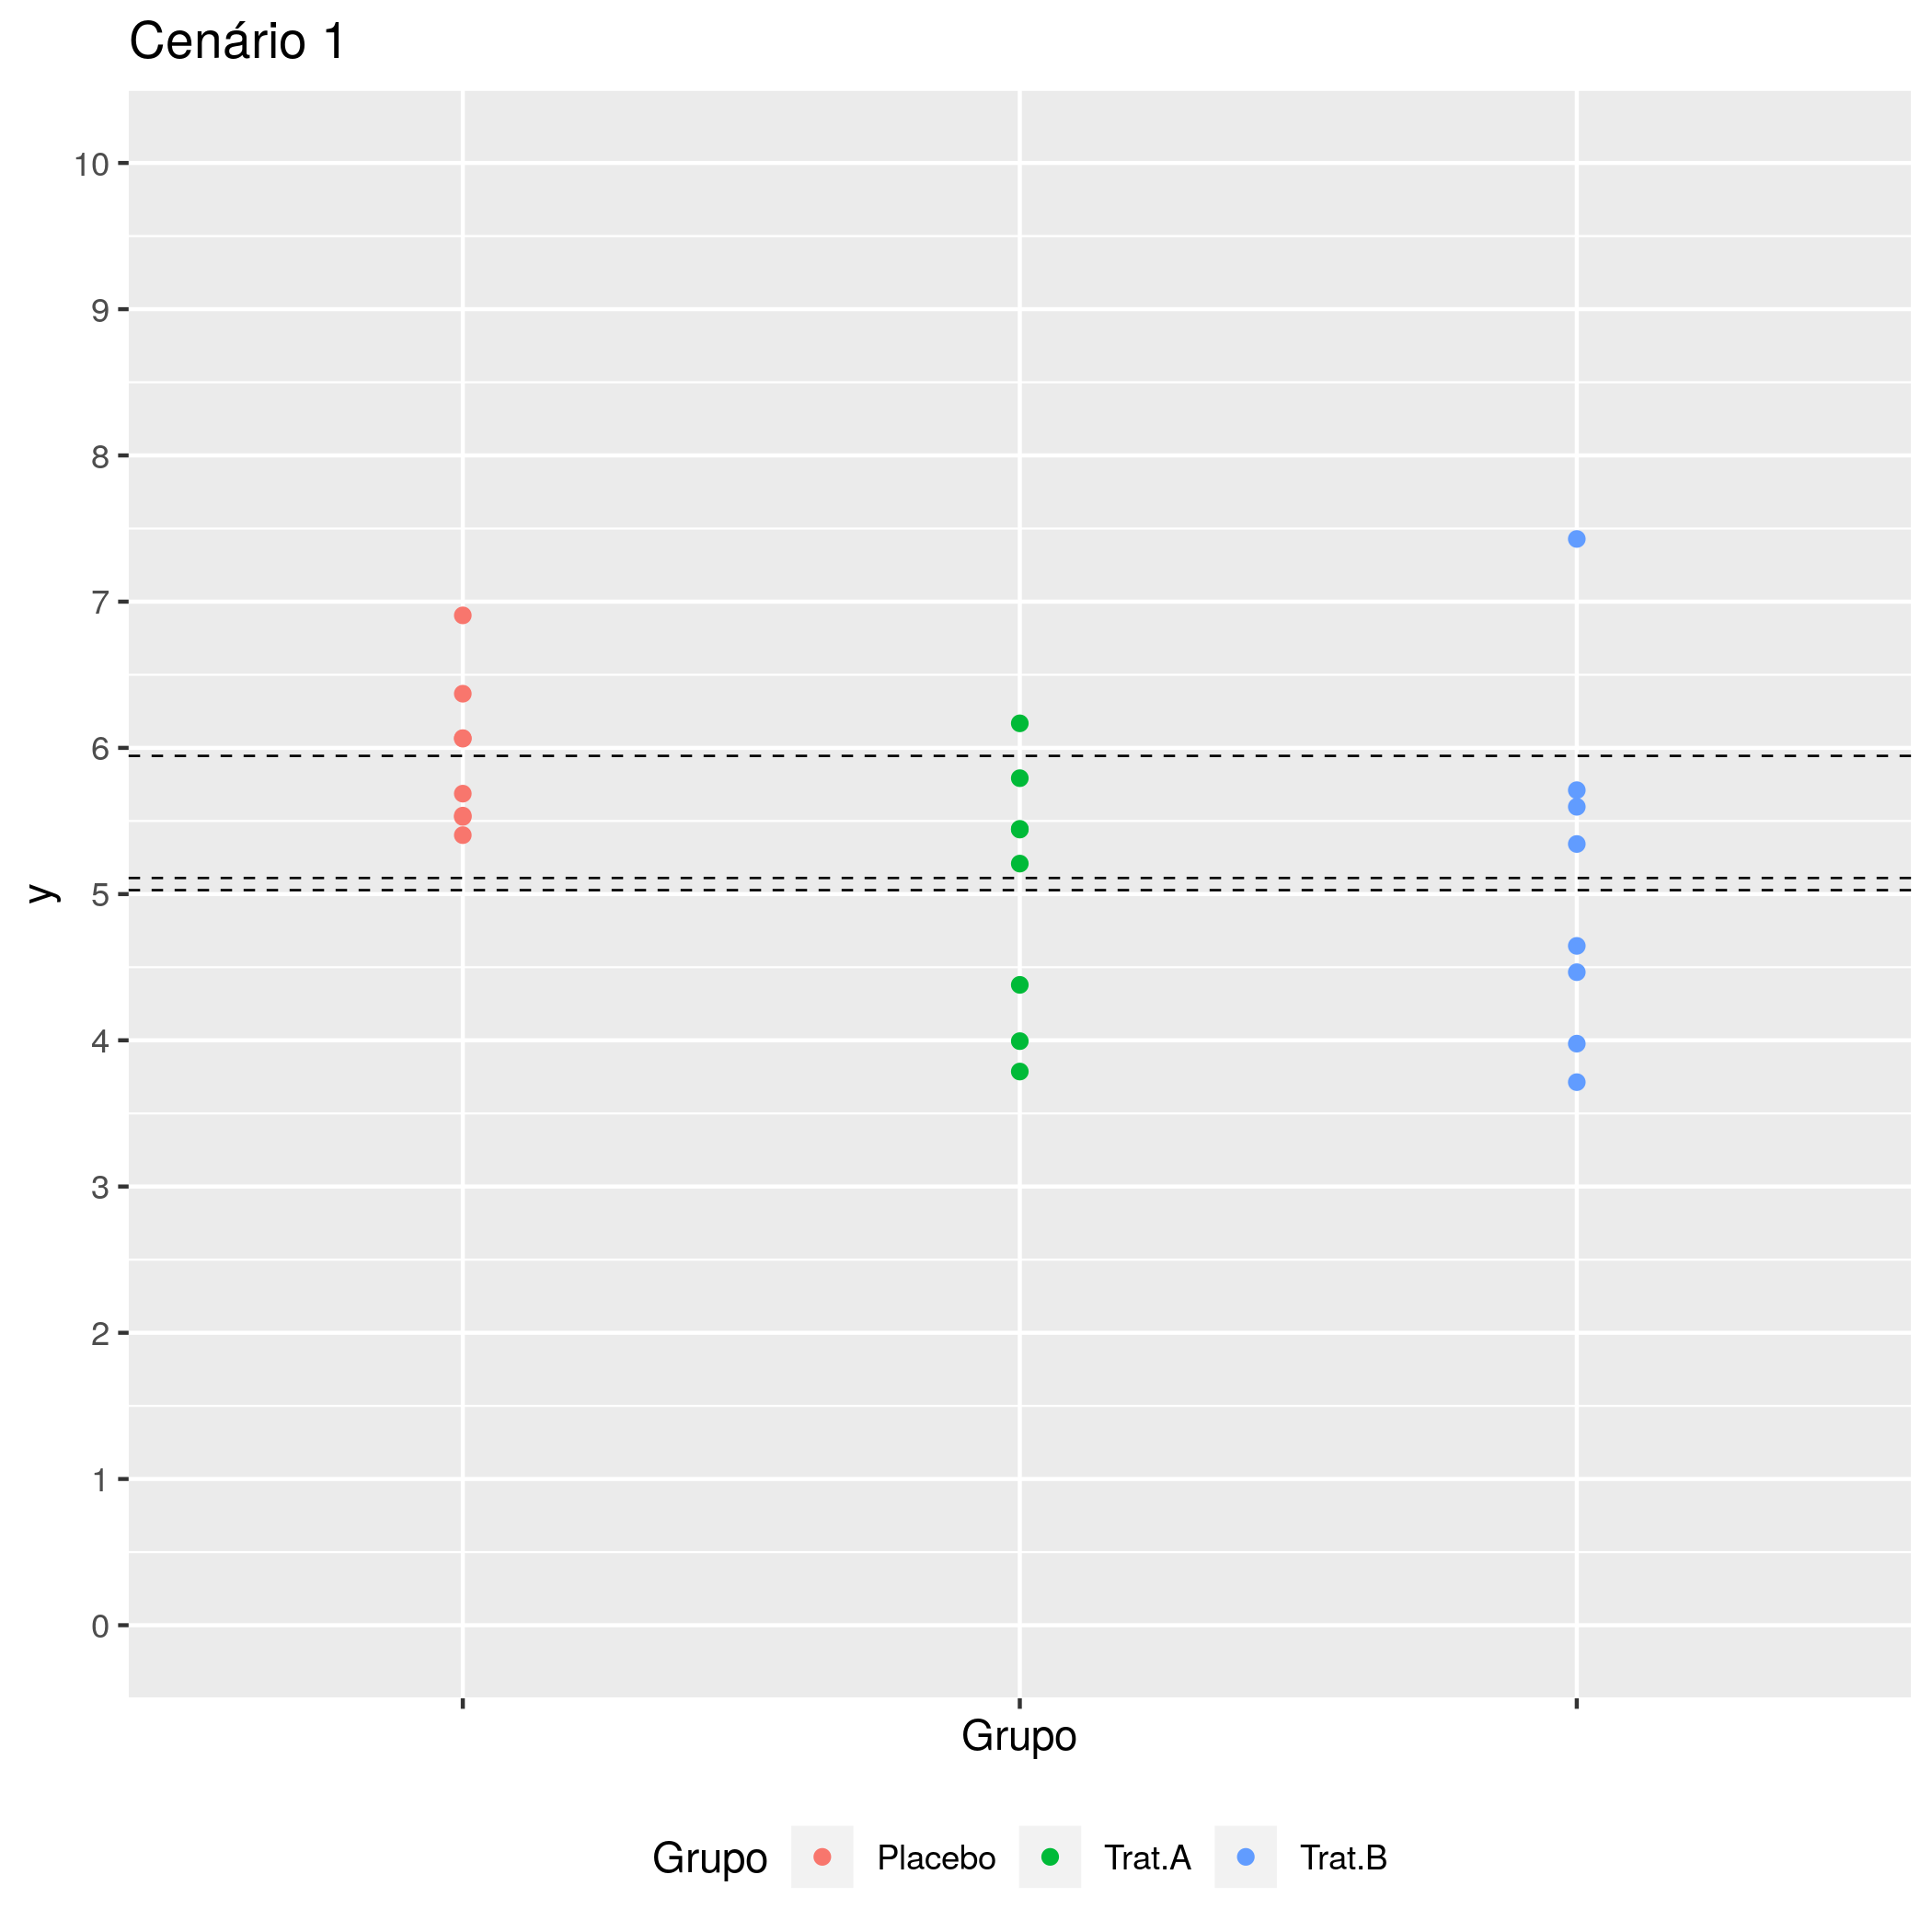
\includegraphics[height=.9\textheight]{Cap13-30/cenario1_medias}

%    {\tiny Médias: Placebo: 4.210, Tratamento A: 3.250, Tratamento B: 3.845}
  \end{center}
\end{frame}

\begin{frame}[label=cenario2]{\small Cenário 2 -- esses 3 grupos têm médias diferentes?}
  \begin{center}
    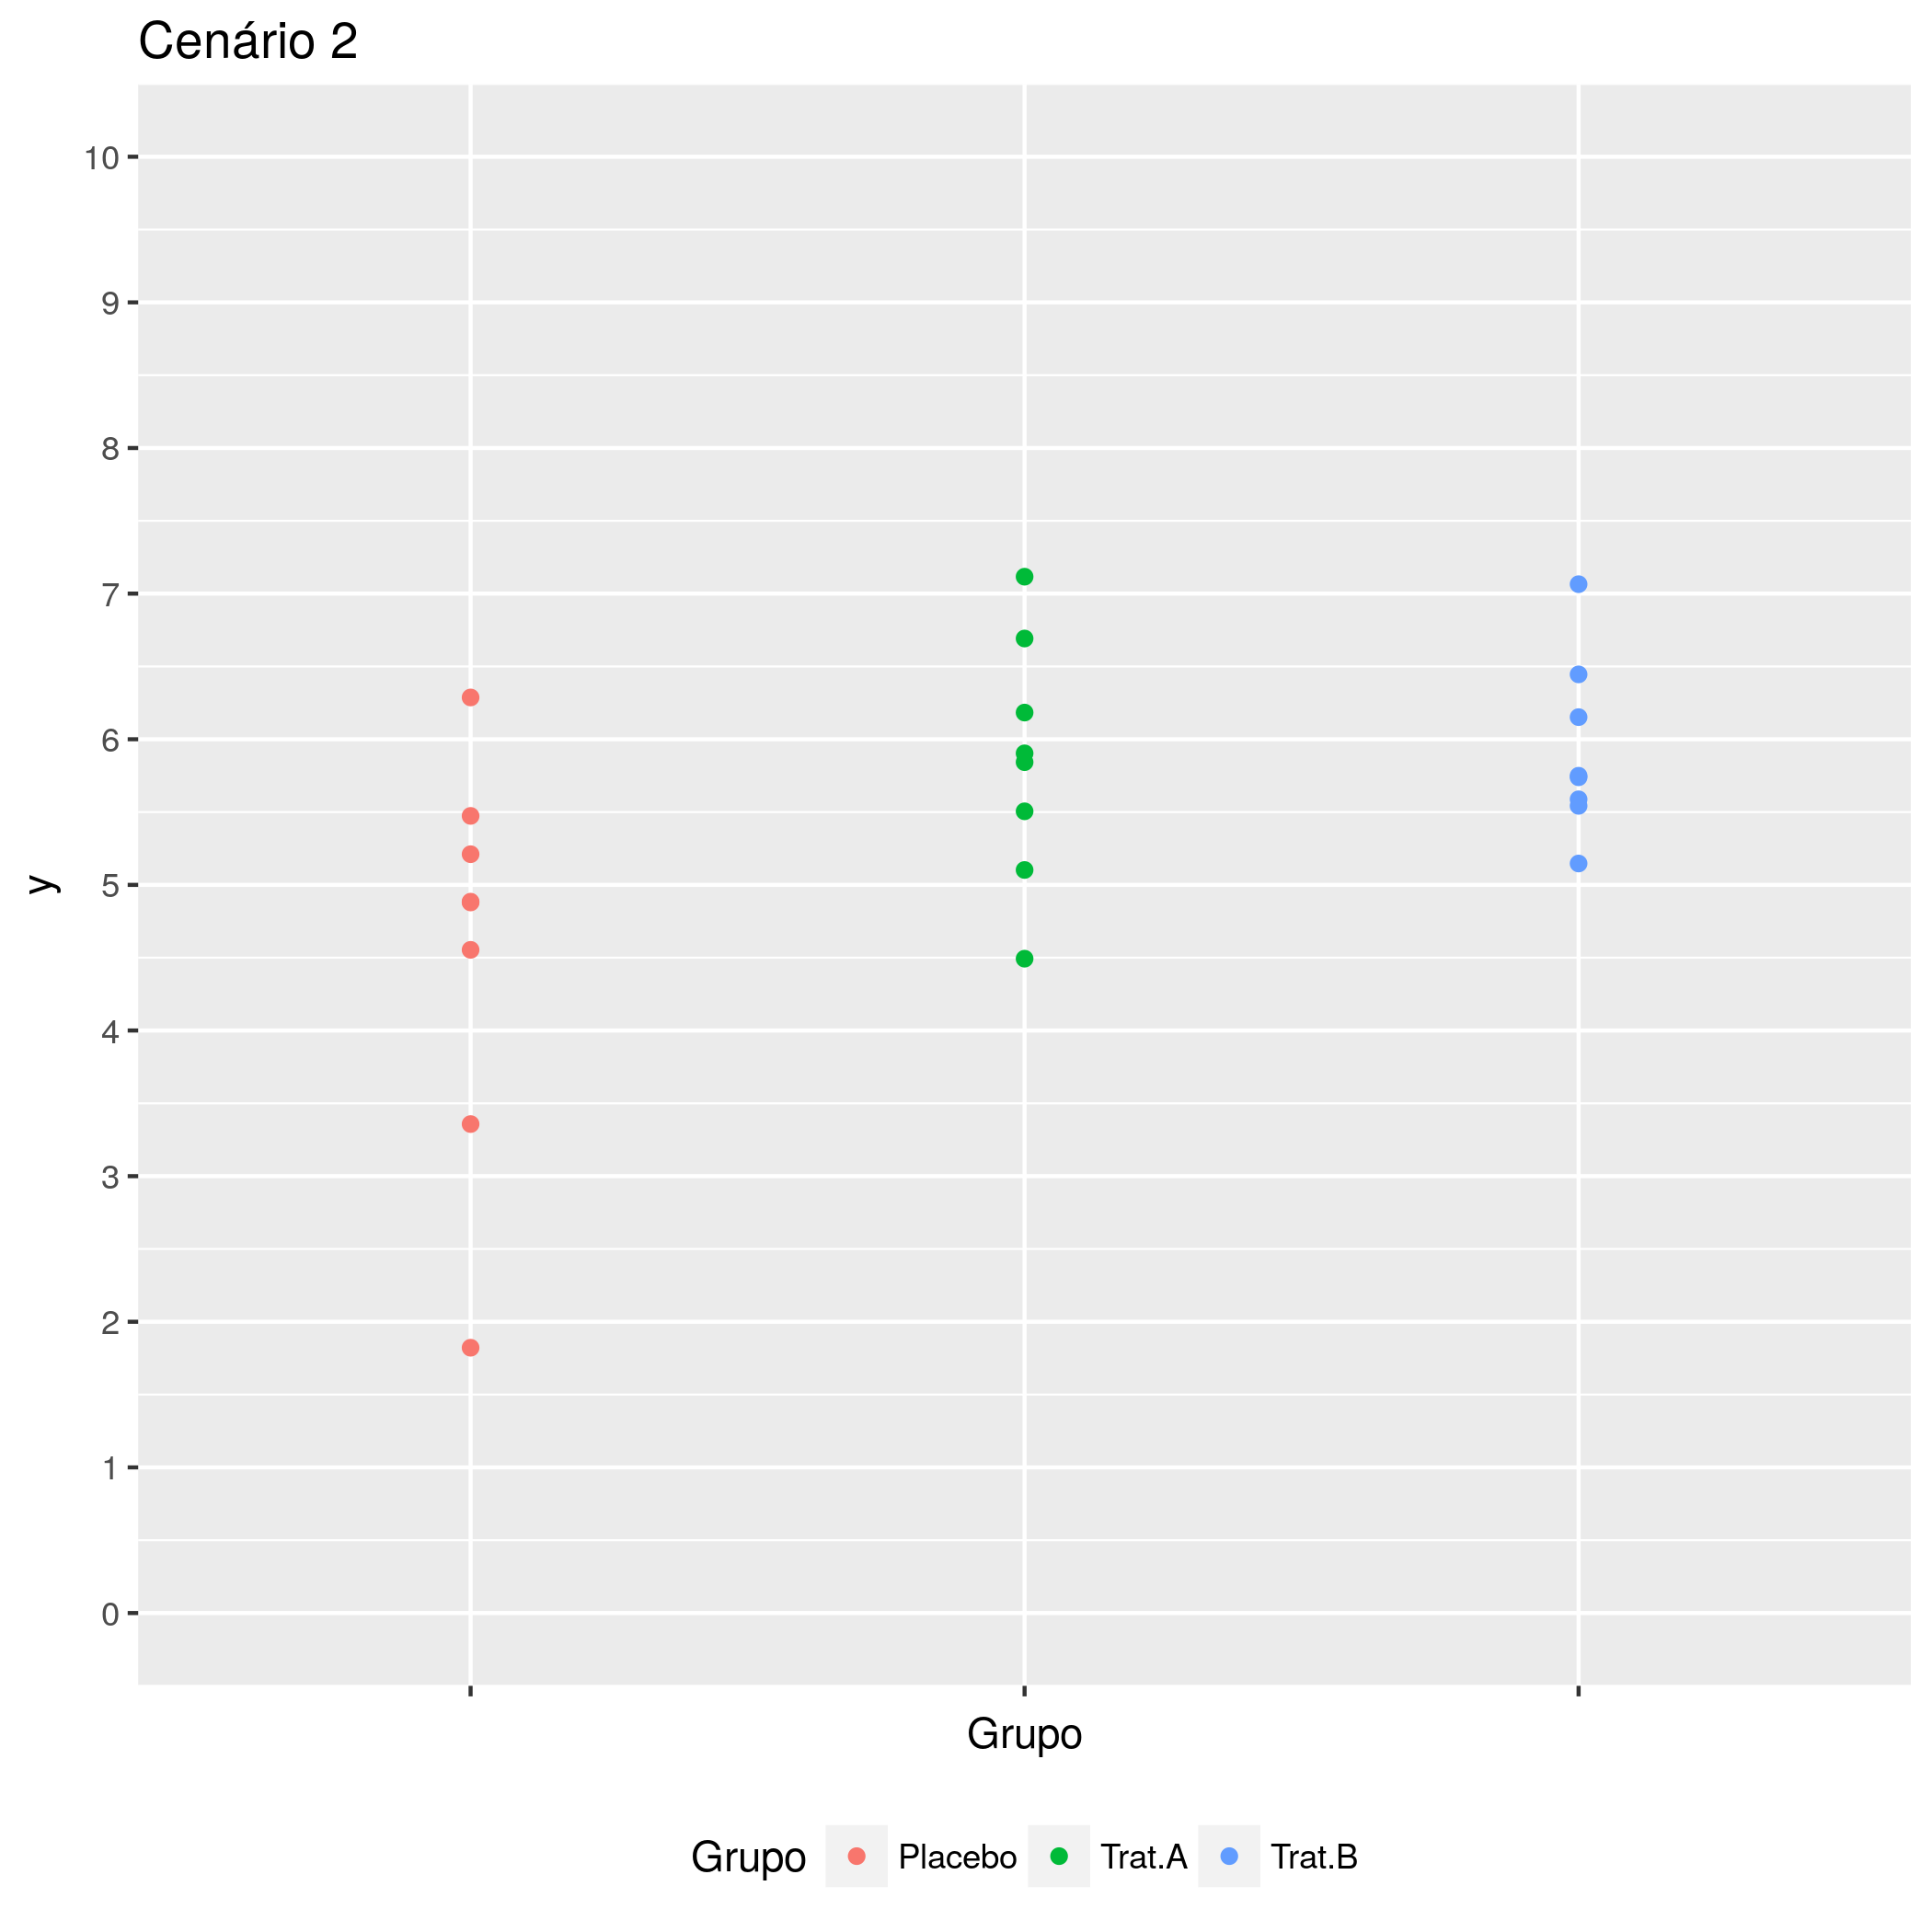
\includegraphics[height=.9\textheight]{Cap13-30/cenario2}
  \end{center}
\end{frame}

\begin{frame}{\footnotesize Médias: Placebo: 3.928, Tratamento A: 6.751, Tratamento B: 5.799}
  \begin{center}
    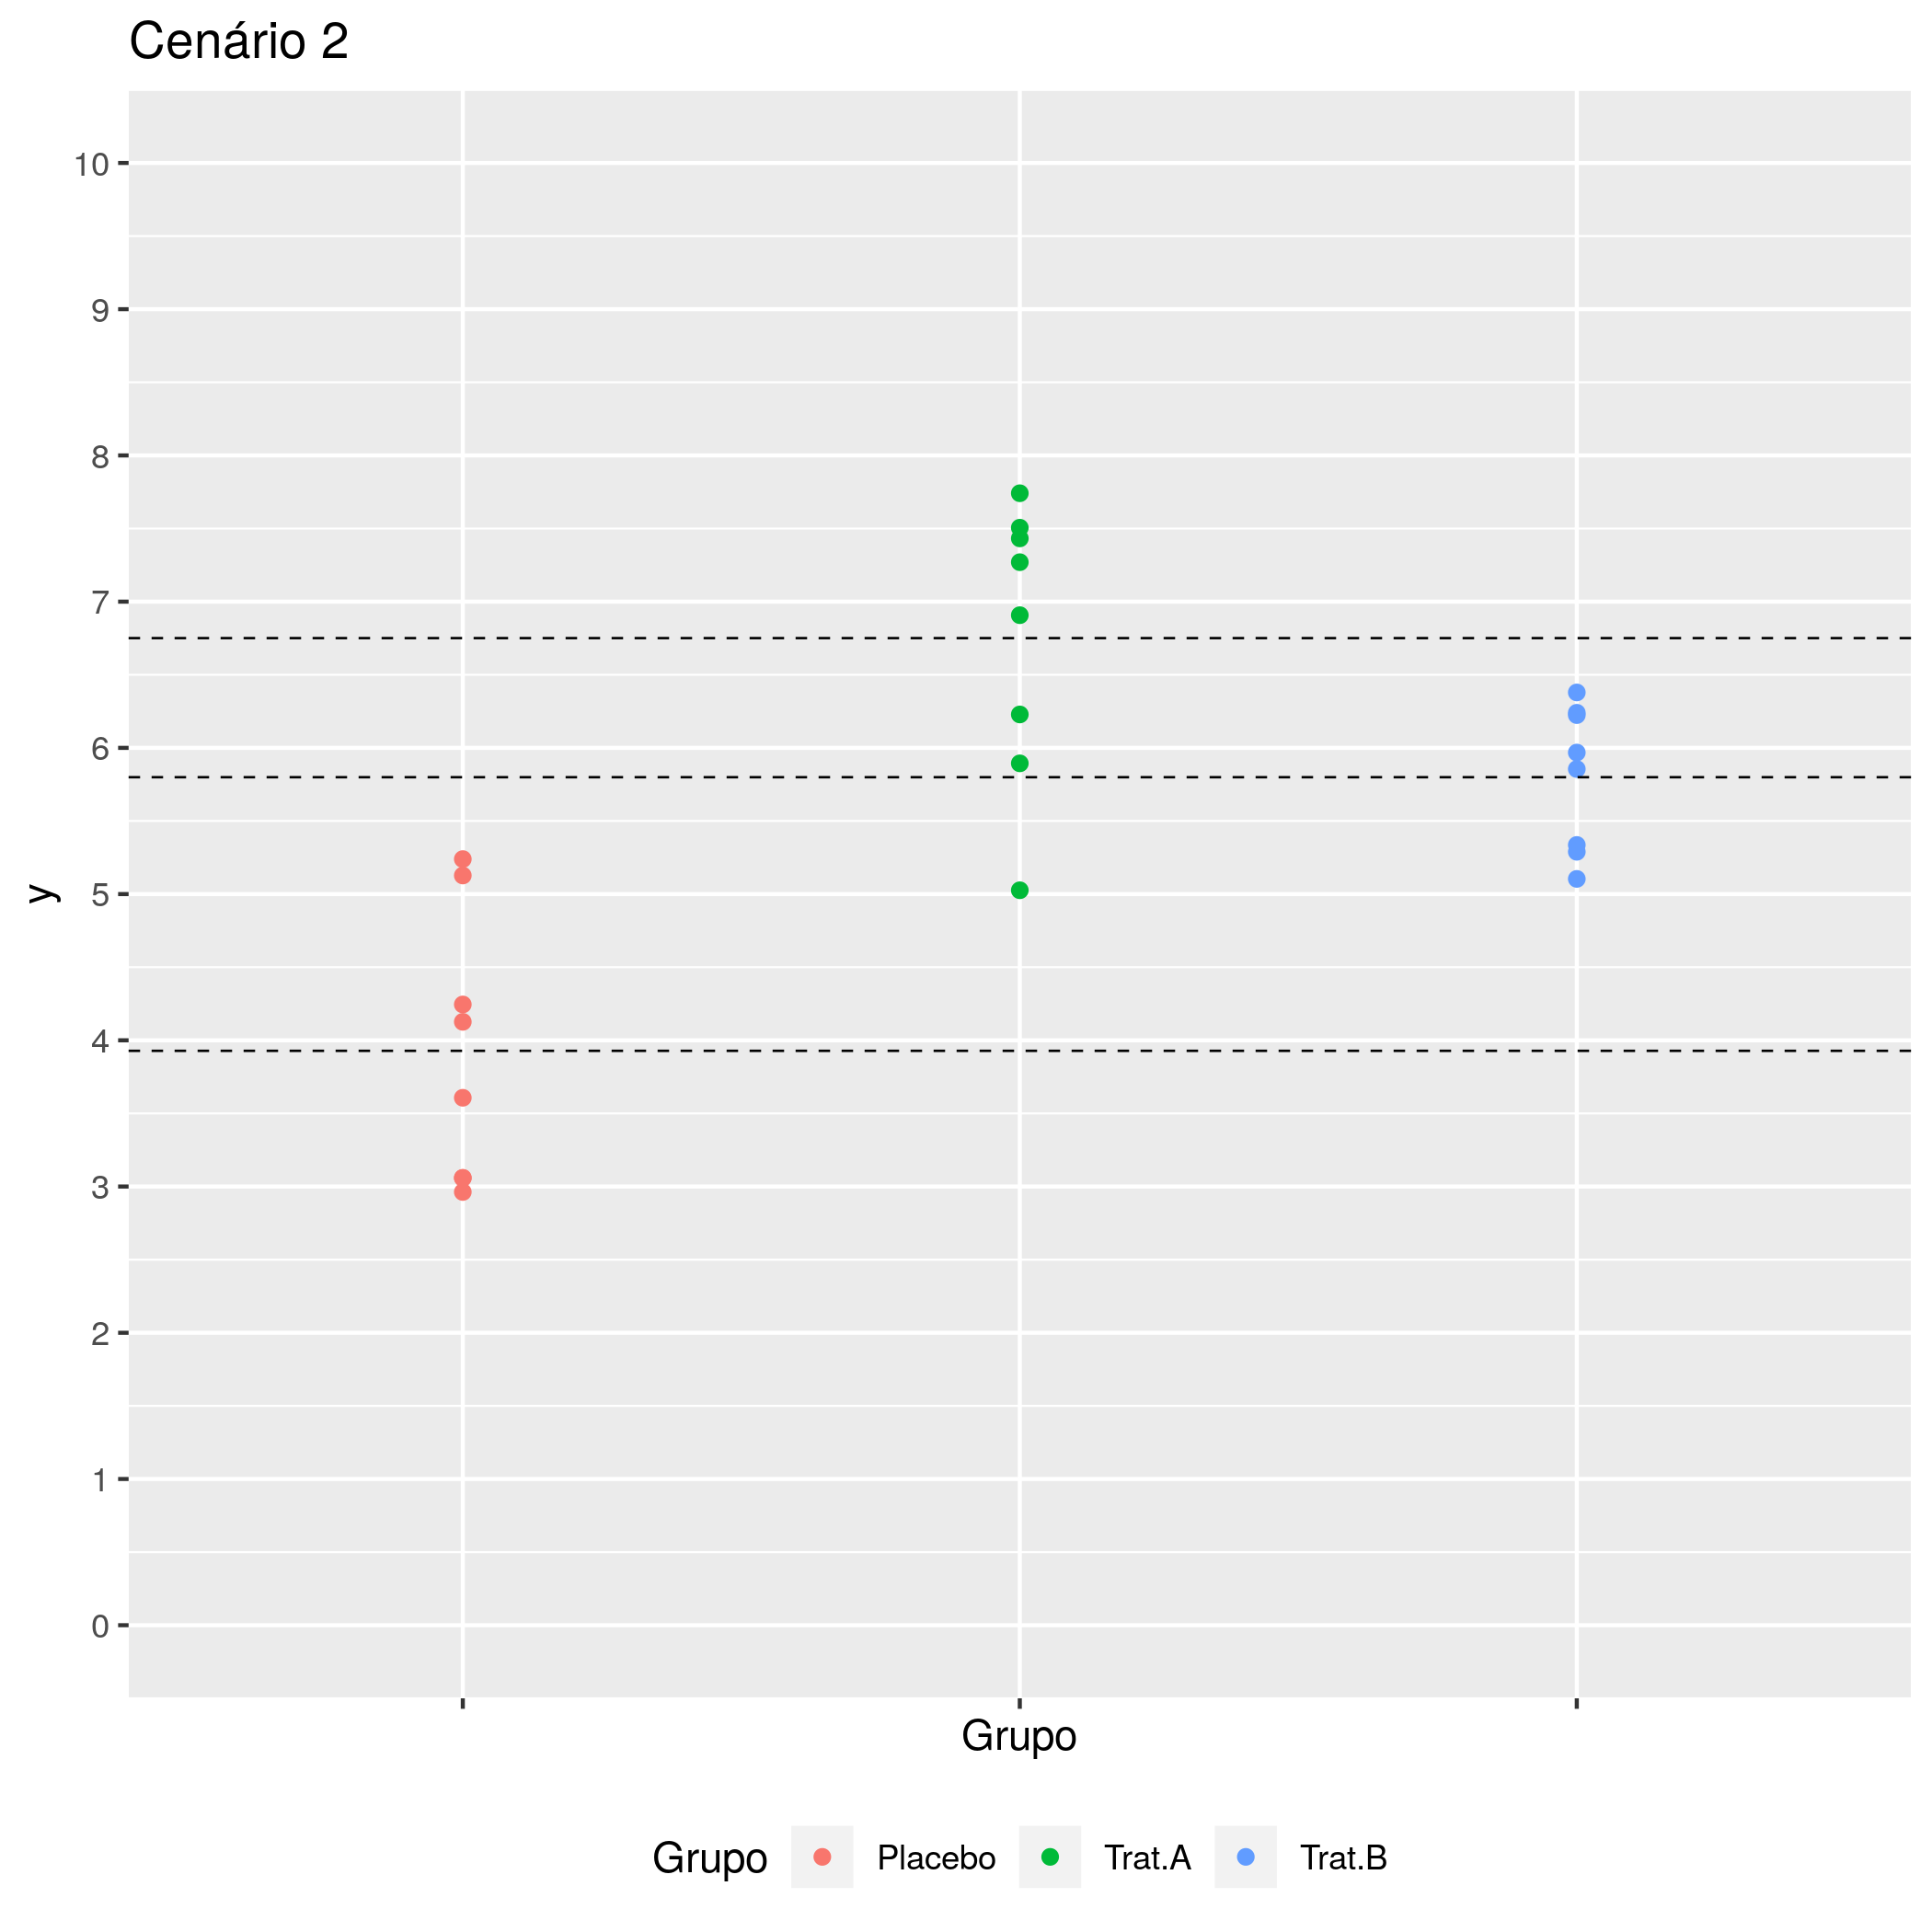
\includegraphics[height=.9\textheight]{Cap13-30/cenario2_medias}

%    {\tiny Médias: Placebo: 4.559, Tratamento A: 5.855, Tratamento B: 5.928}
  \end{center}
\end{frame}

\begin{frame}{\small Comparação entre 3 (ou mais) grupos}
  \begin{block}{Abordagem mais simples}
    \small
    Uma ideia seria usar o teste t três vezes...

    \bigskip
    ... comparando os grupos, dois a dois.
  \end{block}
  \vfill
  \begin{block}{Proposta}
    \begin{enumerate}
      \footnotesize
    \item Placebo x Tratamento A
    \item Placebo x Tratamento B
    \item Tratamento A x Tratamento B
    \end{enumerate}
  \end{block}
\end{frame}

\begin{frame}{\small Cenário 1}
  \begin{columns}
    \begin{column}{5cm}
      \begin{exampleblock}{\footnotesize P-valores dos 3 testes t}
        \begin{enumerate}
          \tiny
        \item Placebo x Trat. A $\Rightarrow p=0.0221$
        \item Placebo x Trat. B $\Rightarrow p=0.0895$
        \item Trat. A x Trat. B $\Rightarrow p=0.8754$
        \end{enumerate}
      \end{exampleblock}
      \bigskip
      \bigskip
      \begin{exampleblock}{\footnotesize Pergunta}
        \small
        Os tratamentos são diferentes do placebo?

        \bigskip
        E entre si?
      \end{exampleblock}
    \end{column}
    \begin{column}{5cm}
      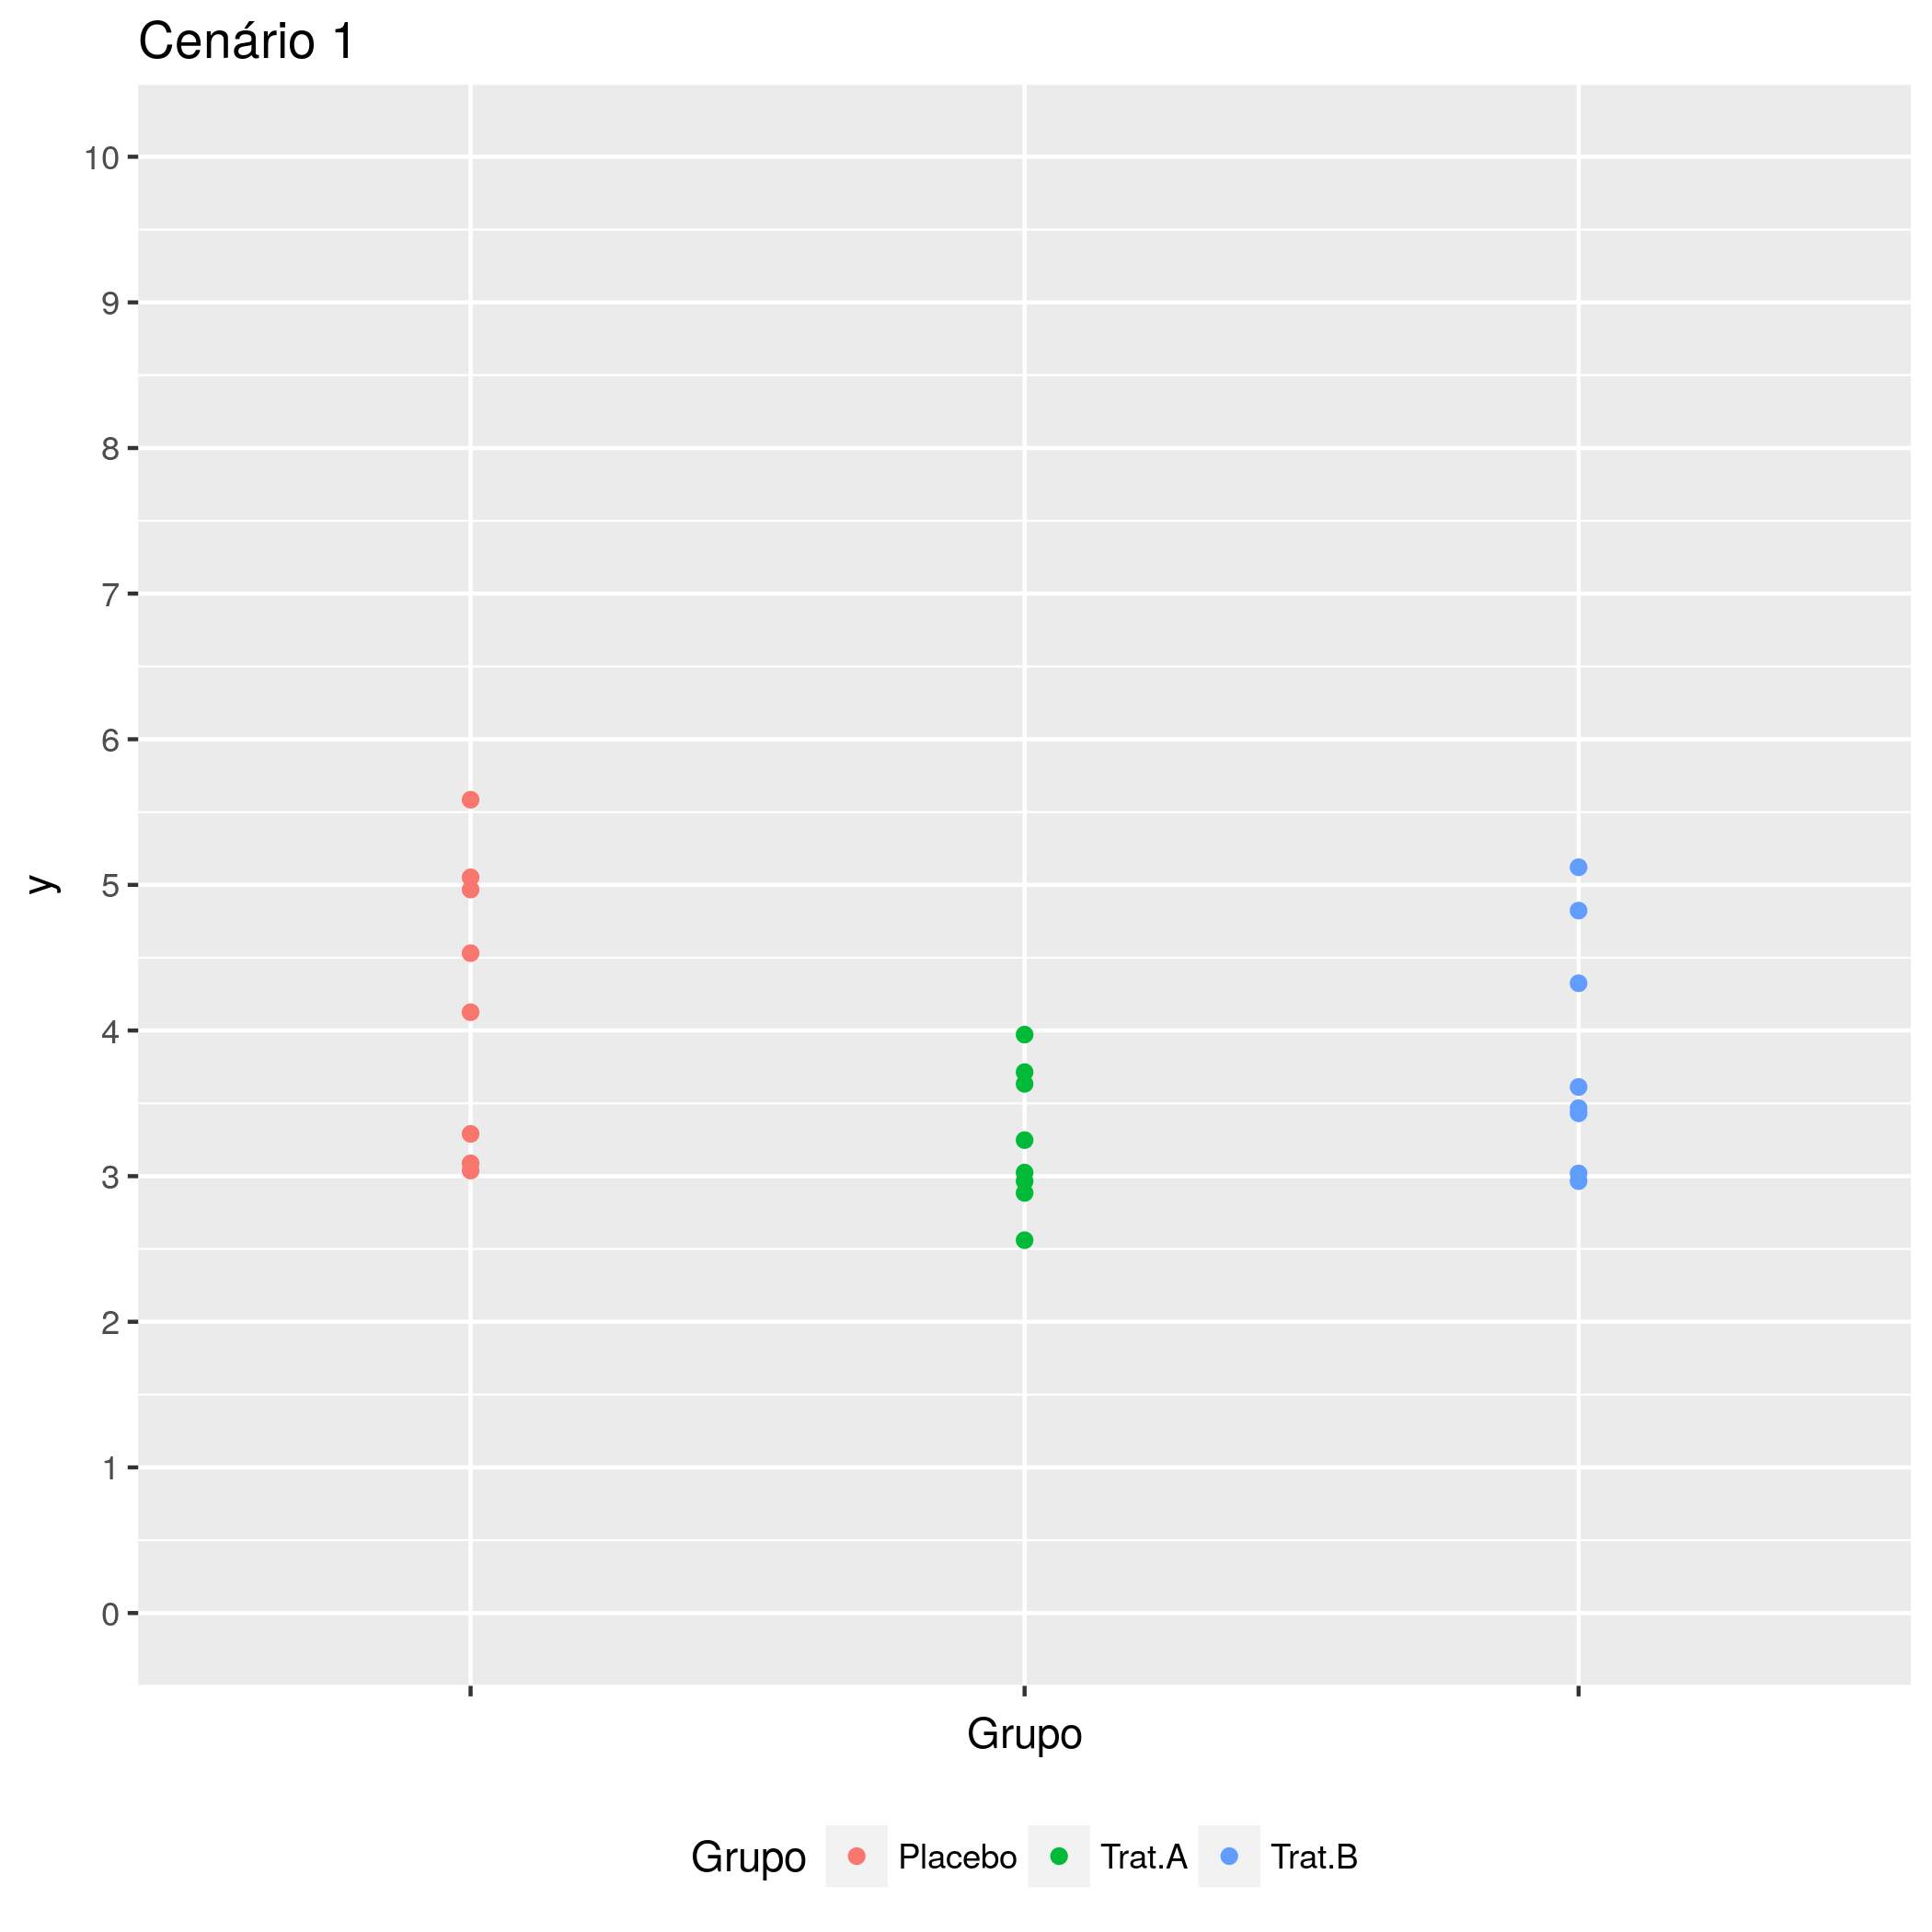
\includegraphics[width=\textwidth]{Cap13-30/cenario1}
    \end{column}
  \end{columns}
\end{frame}

\begin{frame}{\small Cenário 2}
  \begin{columns}
    \begin{column}{5cm}
      \begin{exampleblock}{\footnotesize P-valores dos 3 testes t}
        \tiny
        \begin{enumerate}
        \item Placebo x Trat. A $\Rightarrow p< 0.0001$
        \item Placebo x Trat. B $\Rightarrow p=0.0001622$
        \item Trat. A x Trat. B $\Rightarrow p=0.02459$
        \end{enumerate}
      \end{exampleblock}
      \bigskip
      \bigskip
      \begin{exampleblock}{\footnotesize Pergunta}
        \small
        Os tratamentos são diferentes do placebo?

        \bigskip
        E entre si?
      \end{exampleblock}
    \end{column}
    \begin{column}{5cm}
      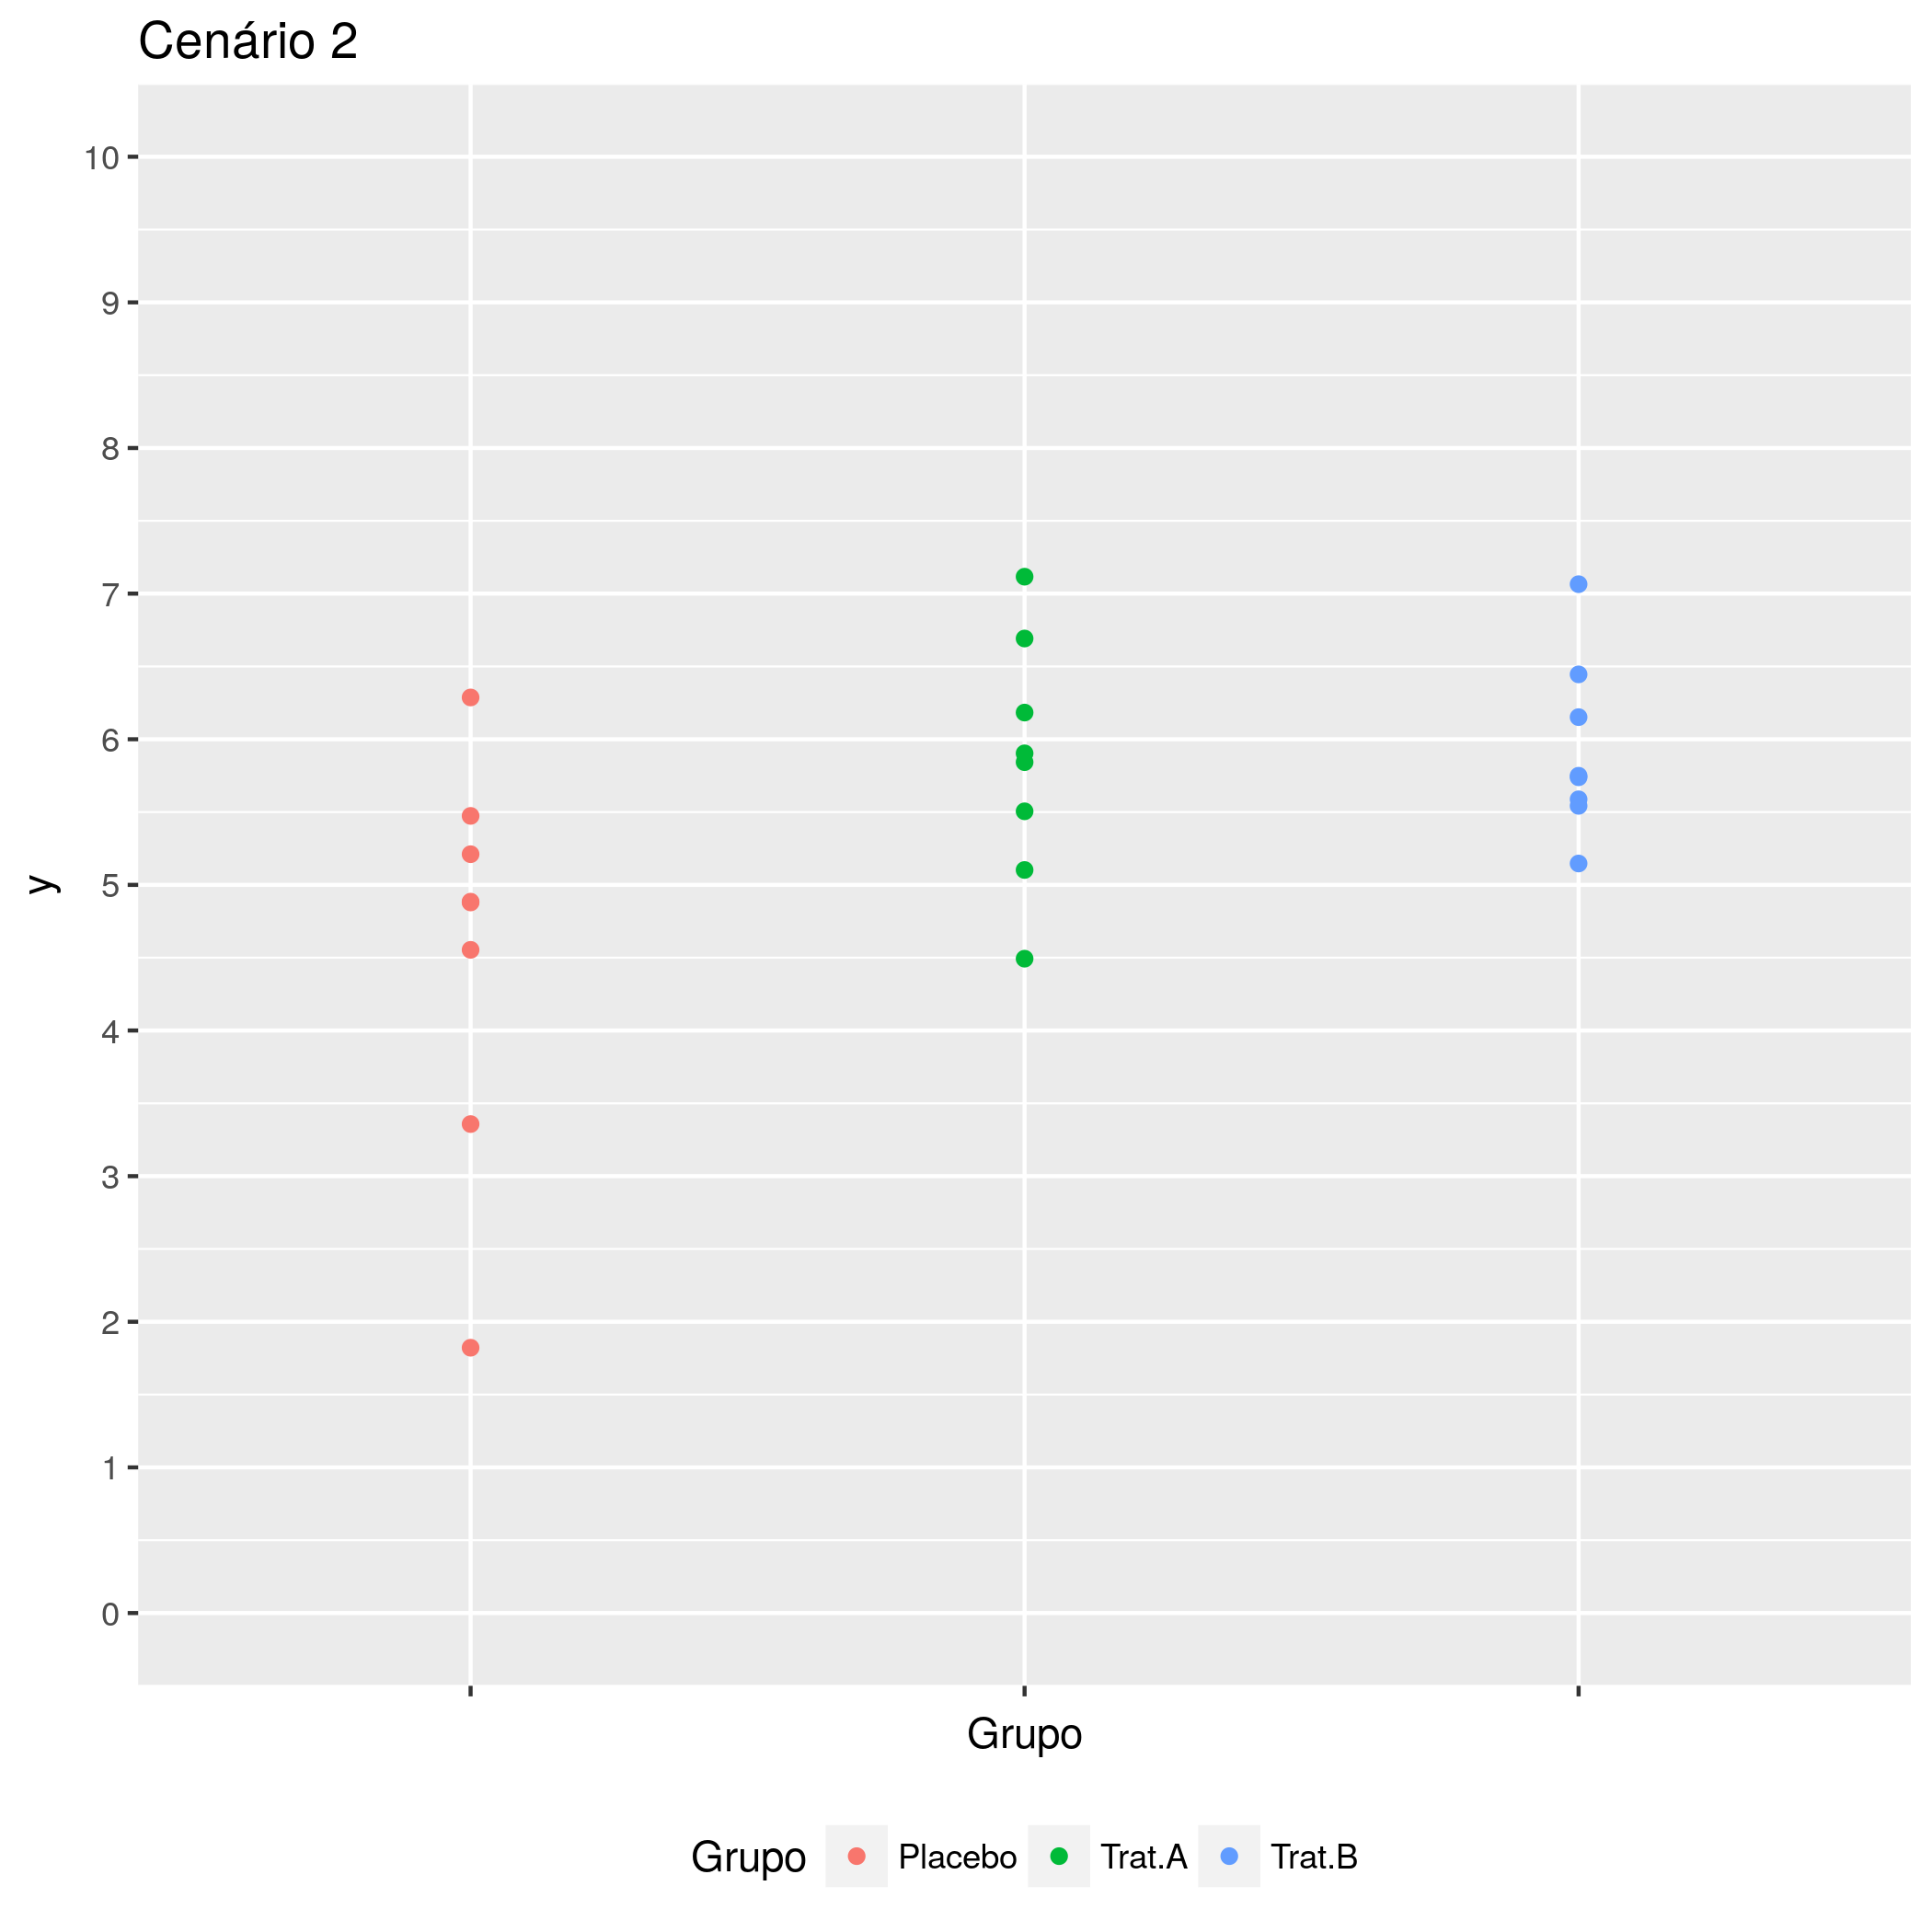
\includegraphics[width=\textwidth]{Cap13-30/cenario2}
    \end{column}
  \end{columns}
\end{frame}

\begin{frame}{}
  \begin{center}
    Existe um problema oculto aí.
  \end{center}
\end{frame}

\begin{frame}{}
  \begin{center}
    O problema é...
  \end{center}
  \begin{block}{}<2->
    \begin{itemize}
      \footnotesize
    \item A conclusão de que no Cenário 1 os 3 grupos são diferentes está {\bf errada}!
    \item No Cenário 2, os 2 tratamentos {\bf não são} diferentes entre si!
    \end{itemize}
  \end{block}
  \medskip
  \bigskip
  \begin{itemize}
    \footnotesize
  \item<3-> O teste t permite a avaliação de {\bf uma} hipótese
  \item<3-> Testamos simultaneamente várias \footnote{Leia várias vezes o Cap 13!}
  \item<3-> Isto aumenta a chance de cometermos um erro tipo I (falso positivo)
  \item<3-> Múltiplos testes superestimam o p-valor do método
  \end{itemize}
\end{frame}

\begin{frame}{\small Pensar é obrigatório}
  \begin{itemize}
    \small
  \item Os testes estatísticos (e fórmulas) não ``sabem'' o que foi levado em conta no estudo.
    \bigskip
    \bigskip
  \item {\em Só o pesquisador sabe}
    % \smallskip
  \item A metodologia da análise precisa levar em conta todo o planejamento do estudo.
  \end{itemize}
\end{frame}

\begin{frame}
  \begin{exampleblock}{Exemplo 13.2}
    \small
    5 crianças de uma escola tiveram leucemia, ano passado.

    \begin{itemize}
    \item Isto é uma coincidência?
    \item Esse agrupamento de casos sugere a presença de toxina ou efeito ambiental que causou a doença?

      \bigskip
      \begin{exampleblock}{}
        Qual é a probabilidade de se observar 5 casos {\em nesta} escola, em um ano?
      \end{exampleblock}
    \end{itemize}
  \end{exampleblock}
\end{frame}

\begin{frame}
  \begin{itemize}
    \footnotesize
  \item Considerando a incidência de leucemia, isto parece ser um dado extraordinário
    \bigskip
    \bigskip
  \item Esta é a pergunta errada, {\em após} observar os casos nesta escola
  \item Se escola não é especial, é preciso considerar outras escolas
    \bigskip
    \bigskip
  \item Além disso, outras doenças (por ex., asma é um fator?)
  \end{itemize}
\end{frame}

\begin{frame}
  \begin{enumerate}
    \footnotesize
  \item Você formulou a hipótese após observar o agrupamento de casos
    \bigskip
  \item Você só destacou a escola por causa do agrupamento
    \bigskip
  \item Agrupamentos ocorrem ao acaso
    \bigskip
  \item Definir população:
    \begin{itemize}
    \item População de escolas (cidade, estado...?)
    \item Tempo de observação (mês, ano, década...?)
    \end{itemize}
  \end{enumerate}
  \begin{block}{}
    \small
    Considerando o tempo, e o número de escolas da população...

    \bigskip
    ... um agrupamento deste tamanho é realmente improvável?
  \end{block}
\end{frame}

\begin{frame}
  \begin{exampleblock}{Exemplo 13.2}
    \footnotesize
    5 crianças de uma escola tiveram leucemia, ano passado.

    \begin{itemize}
    \item Isto é uma coincidência?
    \item Esse agrupamento de casos sugere a presença de toxina ou efeito ambiental que causou a doença?

      \bigskip
      \begin{exampleblock}{}
      \sout{Qual é a probabilidade de se observar 5 casos {\em nesta} escola, em um ano?}
    \end{exampleblock}

    \end{itemize}
  \end{exampleblock}
  \begin{exampleblock}{Pergunta correta}
    \small
    {\bf Qual é a probabilidade de se observar 5 casos {\em em alguma} escola, em um ano?}
  \end{exampleblock}
\end{frame}

\begin{frame}
  \begin{center}
    Coincidências podem ocorrer ao testar múltiplas hipóteses
  \end{center}
\end{frame}

\begin{frame}{E agora, José?}
  \begin{block}{}
    Como levar em conta as comparações múltiplas sem ser induzido ao erro, pelo teste t?
  \end{block}
  \bigskip
  \begin{center}
    
\includegraphics[width=.4\textwidth]{Cap10-11/Jackie-Chan-WTF}
  \end{center}
\end{frame}

\againframe{requisito}

\section[ANOVA]{Análise de Variância (ANOVA)}

\subsection{ANOVA um fator (One-way ANOVA)}

\begin{frame}[label=exemplo13.5-enunciado]{\small Exemplo 13.5}
  \begin{exampleblock}{Exemplo 13.5}
    \small
    Hetland, et. al (1993) pesquisaram alterações hormonais em mulheres corredoras.
    Mediram o nível de hormônio luteinizante (LH) em três grupos:
    \bigskip
    \begin{enumerate}
      \small
    \item sedentárias
    \item corredoras recreacionais
    \item corredoras de elite
    \end{enumerate}
  \end{exampleblock}
\end{frame}

\begin{frame}{Quais são as variáveis?}
  \begin{itemize}
    \small
  \item Dependente:
    \begin{itemize}
      \footnotesize
    \item numérica discreta
    \item numérica contínua
    \end{itemize}
  \item Independente:
    \begin{itemize}
      \footnotesize
    \item grupo (categórica nominal -- 2+ níveis)
    \end{itemize}
  \end{itemize}
  \vfill
  \begin{block}{Esta relação pode ser expressa como}
    \begin{displaymath}
      \text{LH} \sim \text{Grupo}
    \end{displaymath}
  \end{block}
\end{frame}

\begin{frame}[label=exemplo13.5-tabela]{\small Exemplo 13.5}
  \begin{exampleblock}{Exemplo 13.5}
    \begin{center}
      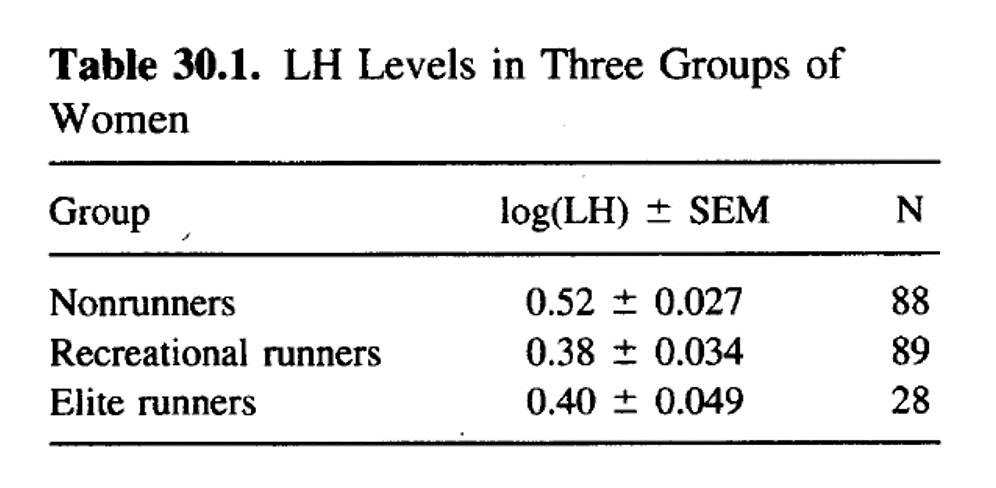
\includegraphics[width=.6\textwidth]{Cap13-30/exemplo13_5-1}
    \end{center}
    \begin{itemize}
      \footnotesize
    \item Com estas informações, podemos construir uma tabela ANOVA
      \small
    \item $H_0$: todas as médias são iguais
    \end{itemize}
  \end{exampleblock}
\end{frame}

\begin{frame}{\small Exemplo 13.5}
  \begin{exampleblock}{Exemplo 13.5}
    \begin{center}
      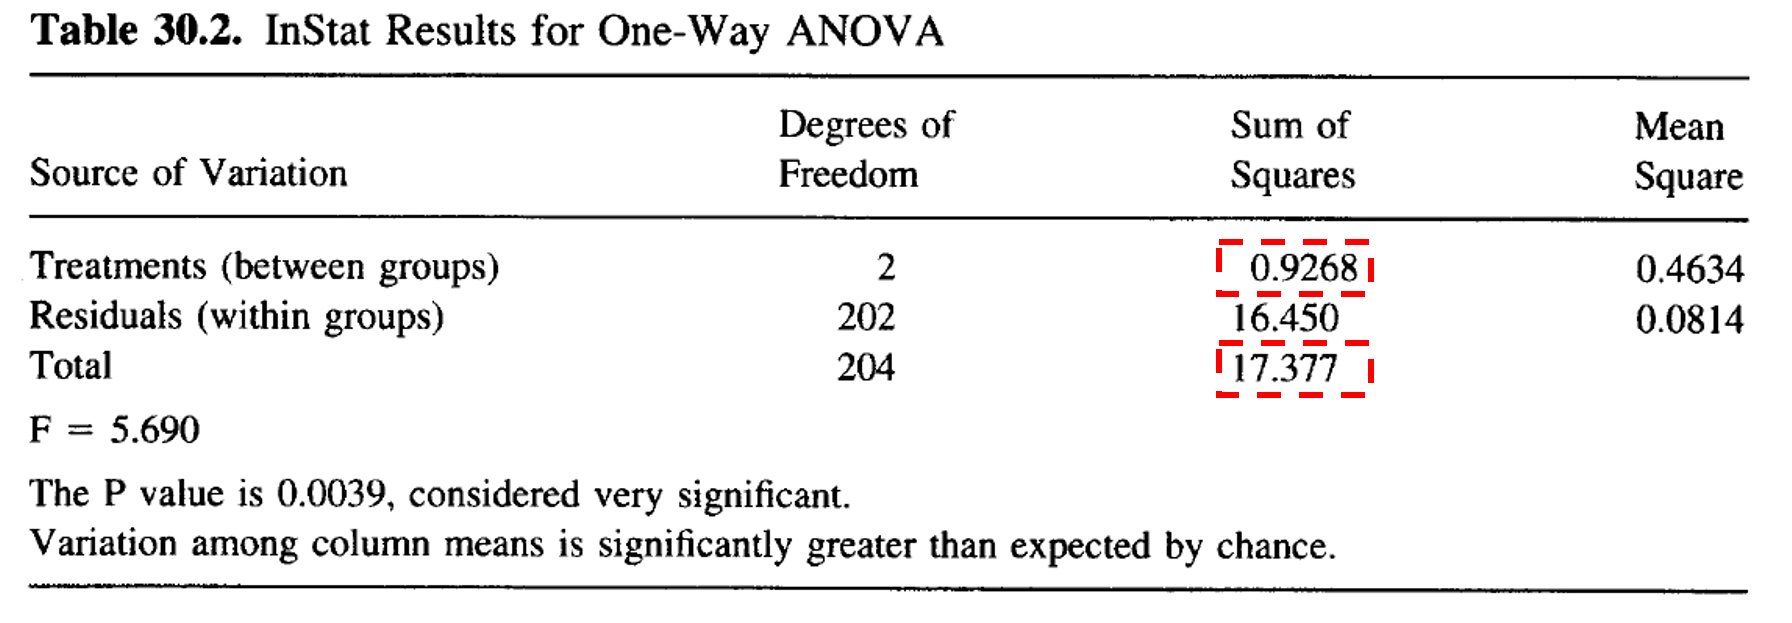
\includegraphics[width=.8\textwidth]{Cap13-30/exemplo13_5-2}
    \end{center}
    \bigskip
    \begin{itemize}
      \scriptsize
    \item A razão entre as Somas dos Quadrados: $0.93/17.38 = 5.3\%$
    \item $5.3\%$ da variabilidade pode ser explicada pelas diferenças {\em entre os grupos}
    \item (lembra do $r^2$?)
    \end{itemize}
  \end{exampleblock}
\end{frame}

\begin{frame}{One-way ANOVA}
  \begin{itemize}
    \small
  \item Este método é chamado one-way (ou 1-way) ANOVA, pois tem um fator categórico
    \bigskip
  \item A premissa é que pode-se {\em modelar} a relação entre um desfecho quantitativo e um preditor categórico + um erro aleatório
    \bigskip
    \bigskip
  \item A variável dependente do exemplo é o LH
  \item A (única) variável independente é o Grupo
  \end{itemize}
\end{frame}

\begin{frame}{A ideia básica}
  \begin{itemize}
    \footnotesize
  \item Quando os grupos têm médias diferentes, parte da variabilidade total é devido a esta diferença
  \item O resto da variabilidade é devido apenas às variâncias intragrupos
  % \item Quando as médias são iguais, temos apenas as variâncias intra-grupos e inter-grupos.
    \bigskip
    \bigskip
  \item A ANOVA tenta {\em desembaraçar} esta decomposição, assumindo a hipótese nula.
  \end{itemize}
\end{frame}

\begin{frame}{A ideia básica}
  \begin{itemize}
    \footnotesize
  \item O nome {\em Análise de Variância} vem do critério usado para comparar as médias
    \bigskip
    \bigskip
  \item O teste é baseado na razão entre as variâncias intra e inter grupos
  \item Estas variâncias aparecem na tabela como ``Média dos Quadrados''
    \bigskip
    \bigskip
  \item Lembrete: a variância é a média dos desvios elevados ao quadrado
  \end{itemize}
\end{frame}

\subsection{O teste F}

\begin{frame}{O teste F\footnote{\scriptsize o teste leva em conta dois graus de liberdade: numerador e denominador} -- expectativa x realidade}
  \begin{block}{}
    \small
    Se as médias forem iguais, a variância intragrupo deve ser ``igual'' à variância intergrupo...

    \bigskip
    ... nesse caso a {\em razão} entre as variâncias deve ser próxima de 1
  \end{block}

  $$F = \frac{\text{variância entre grupos}}{\text{variância intra grupos}}$$

  \begin{block}{Interpretação da estatística $F$}
    Uma razão muito maior que 1 indica que há mais variância entre os grupos do que o esperado
  \end{block}
\end{frame}

\begin{frame}[label=exemplo13.5-anova]{\small Exemplo 13.5}
  \begin{exampleblock}{Exemplo 13.5}
    \begin{center}
      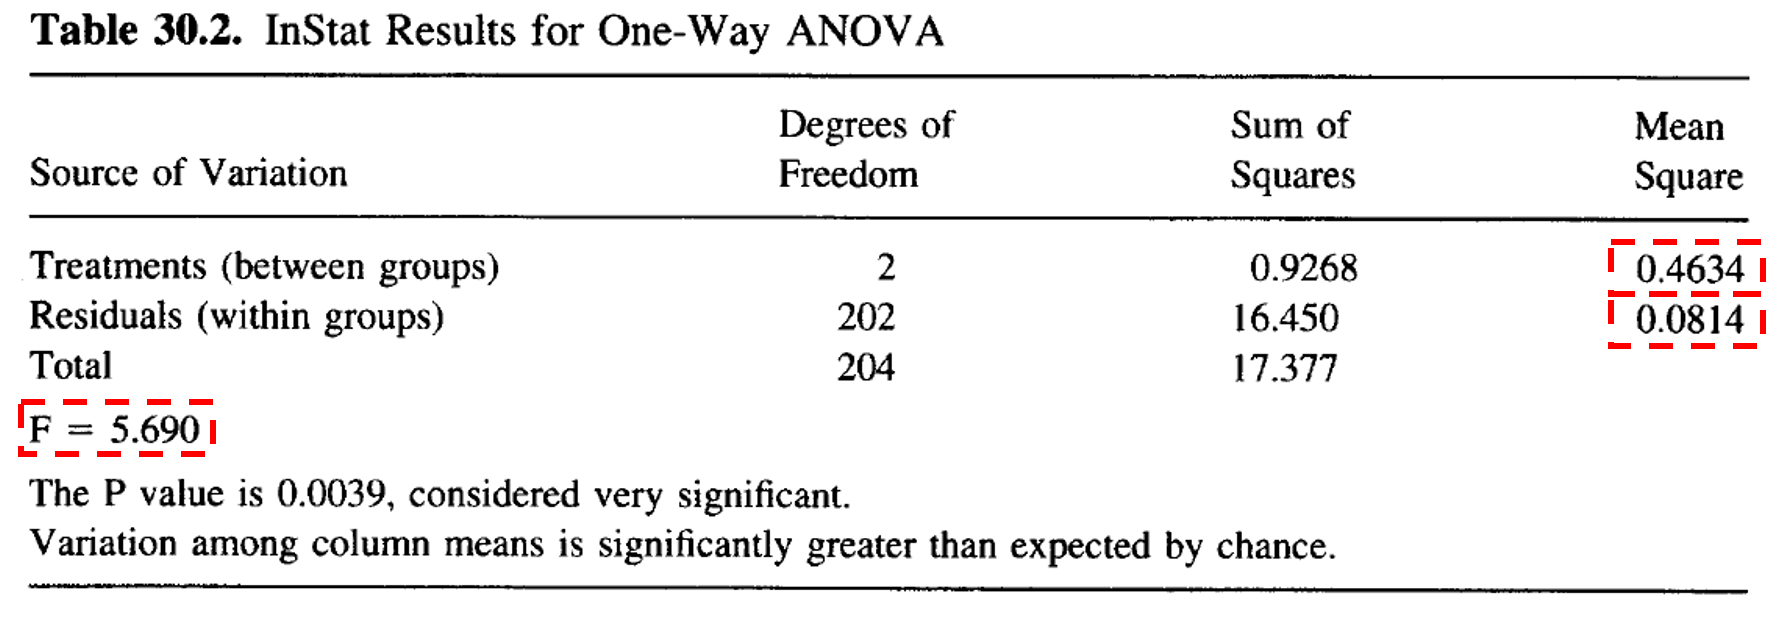
\includegraphics[width=\textwidth]{Cap13-30/exemplo13_5-3}
    \end{center}
    \begin{itemize}
      \scriptsize
    \item Razão entre as variâncias: $F = 0.4634/0.0814 = 5.69 >> 1$

      {\tiny (mesmo considerando o $n$ de cada grupo)}
    \item $p=0.0039$
    \end{itemize}
  \end{exampleblock}
\end{frame}

\begin{frame}{}
  \begin{block}{Resposta}
    Sabemos apenas que pelo menos um dos grupos é diferente dos outros.
    Mas qual(is)?

    \bigskip
    Ainda não estamos prontos para redigir o resultado!
  \end{block}
\end{frame}

\subsection{Pós teste}

\begin{frame}{Testes {\em post-hoc}}
  \begin{itemize}
    \footnotesize
  \item O teste de ANOVA é apenas a primeira parte!\footnote{Está com saudade do teste t?}
    \bigskip
    \bigskip
    \begin{block}{}
      O p-valor do teste F indica o quão raro é encontrar uma discrepância tão grande (ou maior) entre as médias dos grupos, ao acaso
    \end{block}
    \bigskip
    \bigskip
  \item Mas isso não nos ajuda a saber {\bf qual} é o grupo discrepante
  \item Para esta outra pergunta, precisamos de outro método
  \end{itemize}
\end{frame}

\begin{frame}{Testes {\em post-hoc}}
  \begin{itemize}
    \footnotesize
  \item Como vimos, não podemos simplesmente fazer vários testes t
    \bigskip
    \bigskip
  \item Mas podemos {\em ajustar} os p-valores destes testes, para compensar a {\em inflação} destes resultados
    \bigskip
    \bigskip
  \item Isso pode ser feito de várias maneiras
  \end{itemize}
\end{frame}

\begin{frame}{Testes {\em post-hoc}}
  \begin{itemize}
    \small
  \item {\bf Correção de Bonferroni}
  \item Correção para tendências
  \item {\bf Teste ``honesto'' das diferenças, de Tukey (HSD)}
  \item Método de Scheffe
  \item Teste de Dunnet
  \item etc.
  \end{itemize}
\end{frame}

\begin{frame}{Ajustando os p-valores}
  \begin{itemize}
    \footnotesize
  \item Faremos os múltiplos testes t, com ajuste de p-valor
  \item Os dois mais usados são Bonferroni e Tukey
%  \item O teste de Bonferroni é mais simples, e tem mais sensibilidade (com menos especificidade)
%  \item O teste de Tukey tem mais especificidade, mas menos sensibilidade
    \bigskip
    \bigskip
 \item O ajuste de Bonferroni multiplica o p-valor pelo número de comparações, mas seus ICs são muito grandes
    \bigskip
 \item O ajuste de Tukey é mais conservador, mas pode acusar diferenças significativas com mais frequência
    \bigskip
    \bigskip
 \item Infelizmente não há consenso sobre critérios de escolha
  \end{itemize}
\end{frame}

\againframe{exemplo13.5-enunciado}
\againframe{exemplo13.5-tabela}
\againframe{exemplo13.5-anova}

\begin{frame}{\small Exemplo 13.5 -- testes t com ajuste de Tukey}
  \begin{exampleblock}{Exemplo 13.5}
    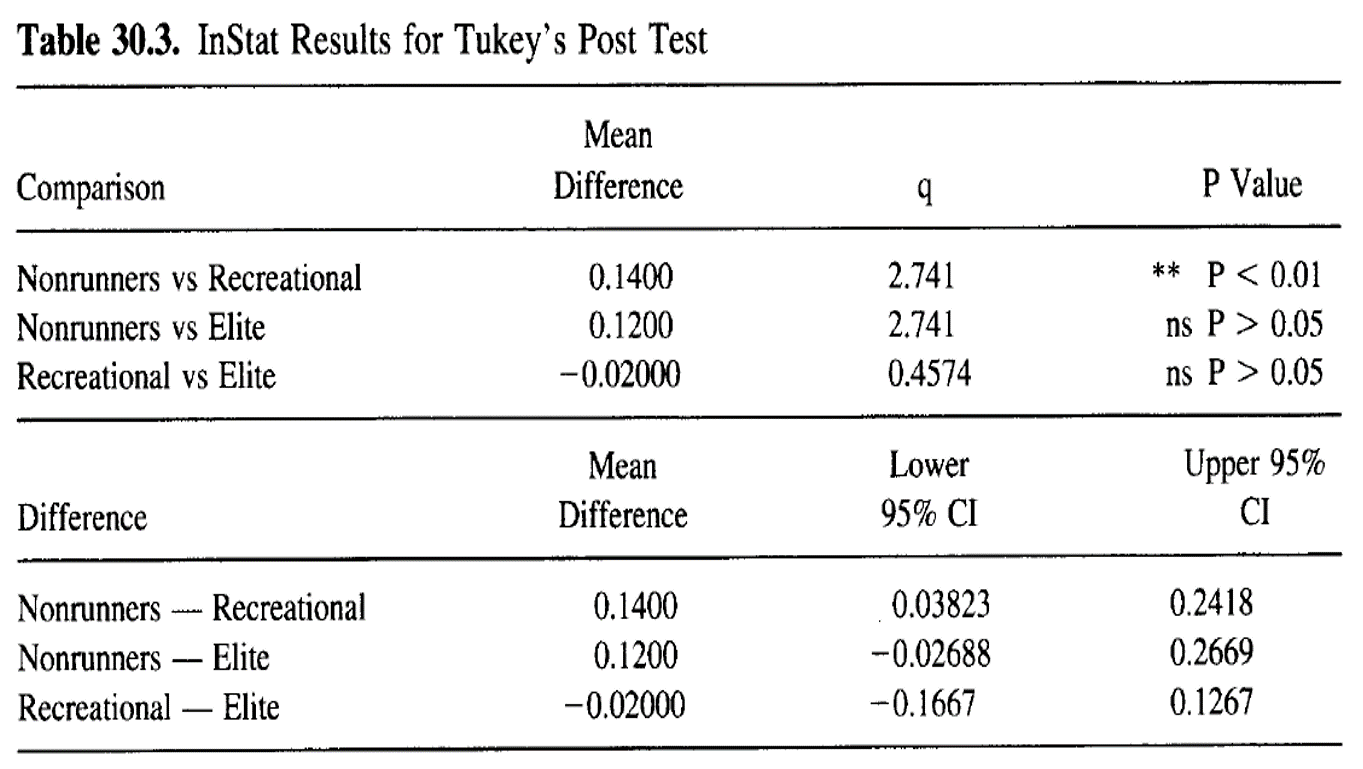
\includegraphics[width=\textwidth]{Cap13-30/exemplo13_5-4}
  \end{exampleblock}
  \begin{block}{Pergunta}
    Como você redigiria este resultado?
  \end{block}
\end{frame}

\subsection{Two-way ANOVA}

\begin{frame}{ANOVA dois parâmetros}
  \begin{itemize}
    \footnotesize
  \item Vimos como usar o ANOVA com {\bf uma} var. independente categórica
    \bigskip
  \item O teste ANOVA permite qualquer quantidade de variáveis independentes! E de qualquer tipo\footnote{\scriptsize Na verdade, ANOVA e Regressão Linear são Múltipla são siameses}
    \bigskip
    \bigskip
  \item Vejamos o exemplo inicial da aula, com duas var. independentes
  \end{itemize}
  \begin{block}{Nova pergunta}
    \small
    Os tratamentos são diferentes, mesmo controlando pelo Gênero?
  \end{block}
\end{frame}

\begin{frame}{Quais são as variáveis?}
  \begin{itemize}
    \small
  \item Dependente:
    \begin{itemize}
      \footnotesize
    \item numérica discreta
    \item numérica contínua
    \end{itemize}
  \item Independentes:
    \begin{itemize}
      \footnotesize
    \item grupo (categórica nominal -- 2+ níveis)
    \end{itemize}
  \end{itemize}
  \vfill
  \begin{block}{Esta relação pode ser expressa como}
    \begin{displaymath}
      \text{Mensuração} \sim \text{Grupo de tratamento} \alert{+ \text{Gênero}}
    \end{displaymath}
  \end{block}
\end{frame}

\againframe{cenario1}

\begin{frame}[label=cenario3]{\small Cenário 3 = cenário 1 ajustando pelo Gênero}
  \begin{center}
    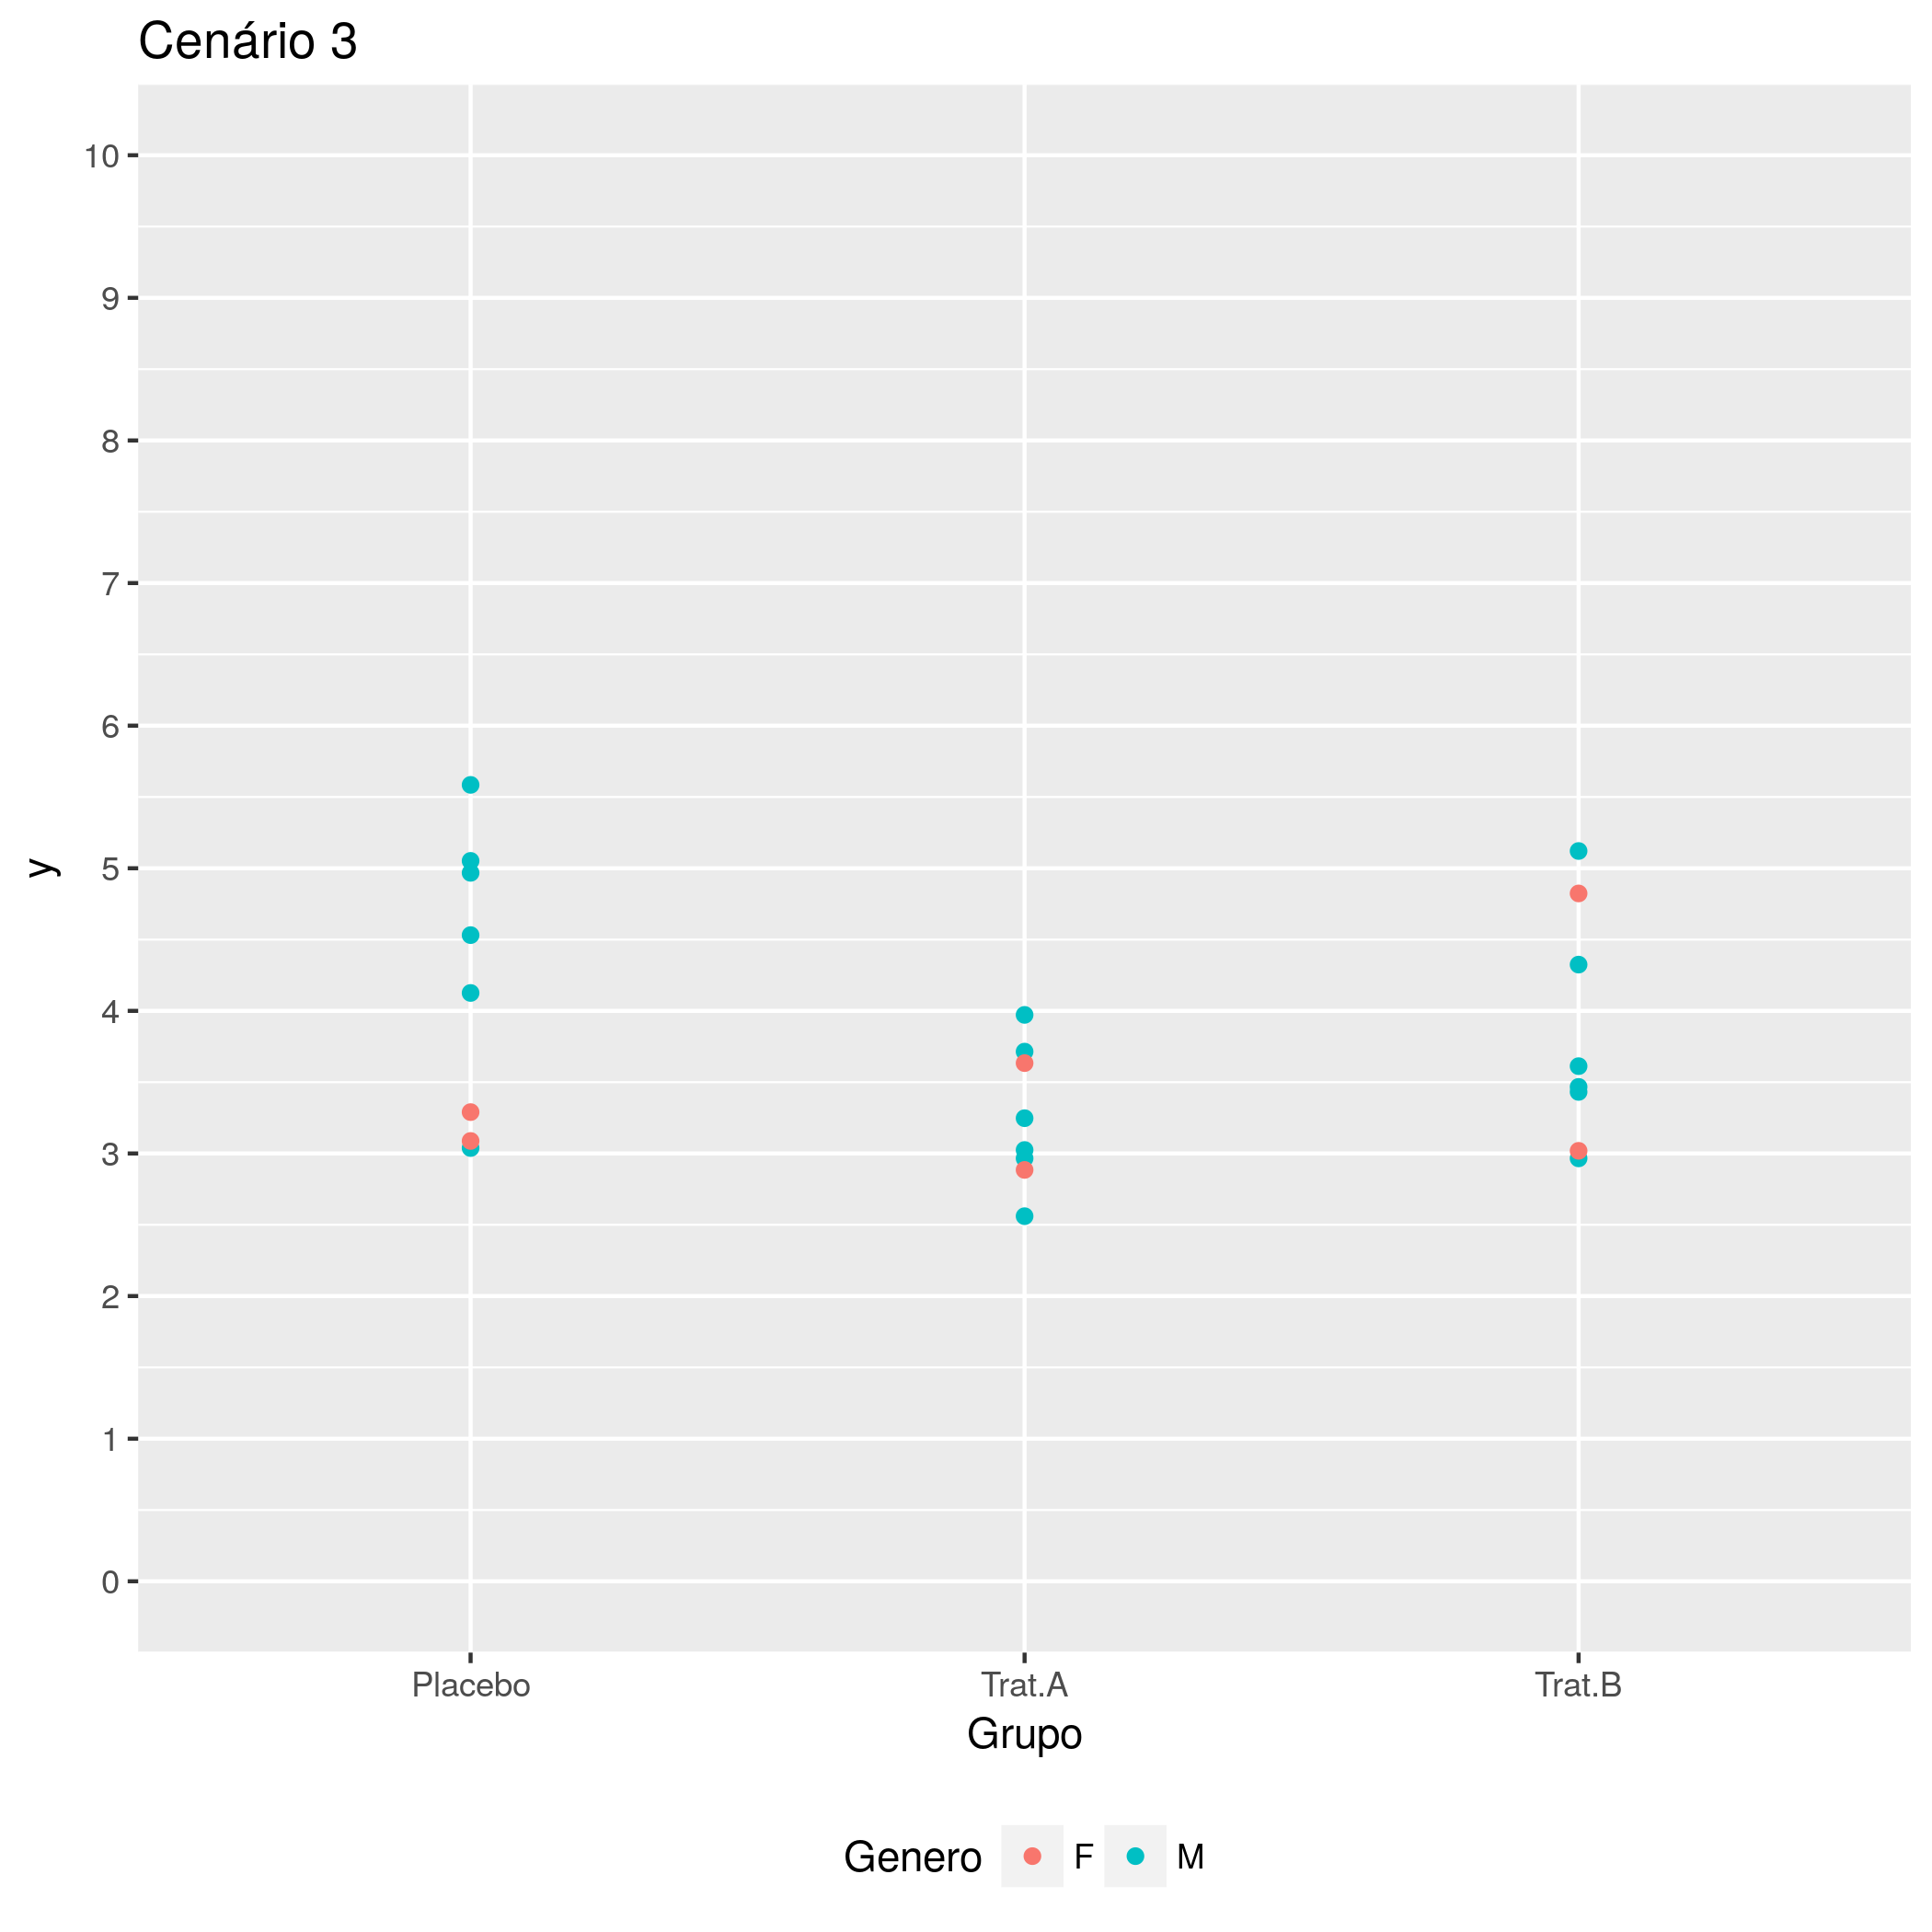
\includegraphics[height=.9\textheight]{Cap13-30/cenario12}
  \end{center}
\end{frame}

\againframe{cenario2}

\begin{frame}[label=cenario4]{\small Cenário 4 = cenário 2 ajustando pelo Gênero}
  \begin{center}
    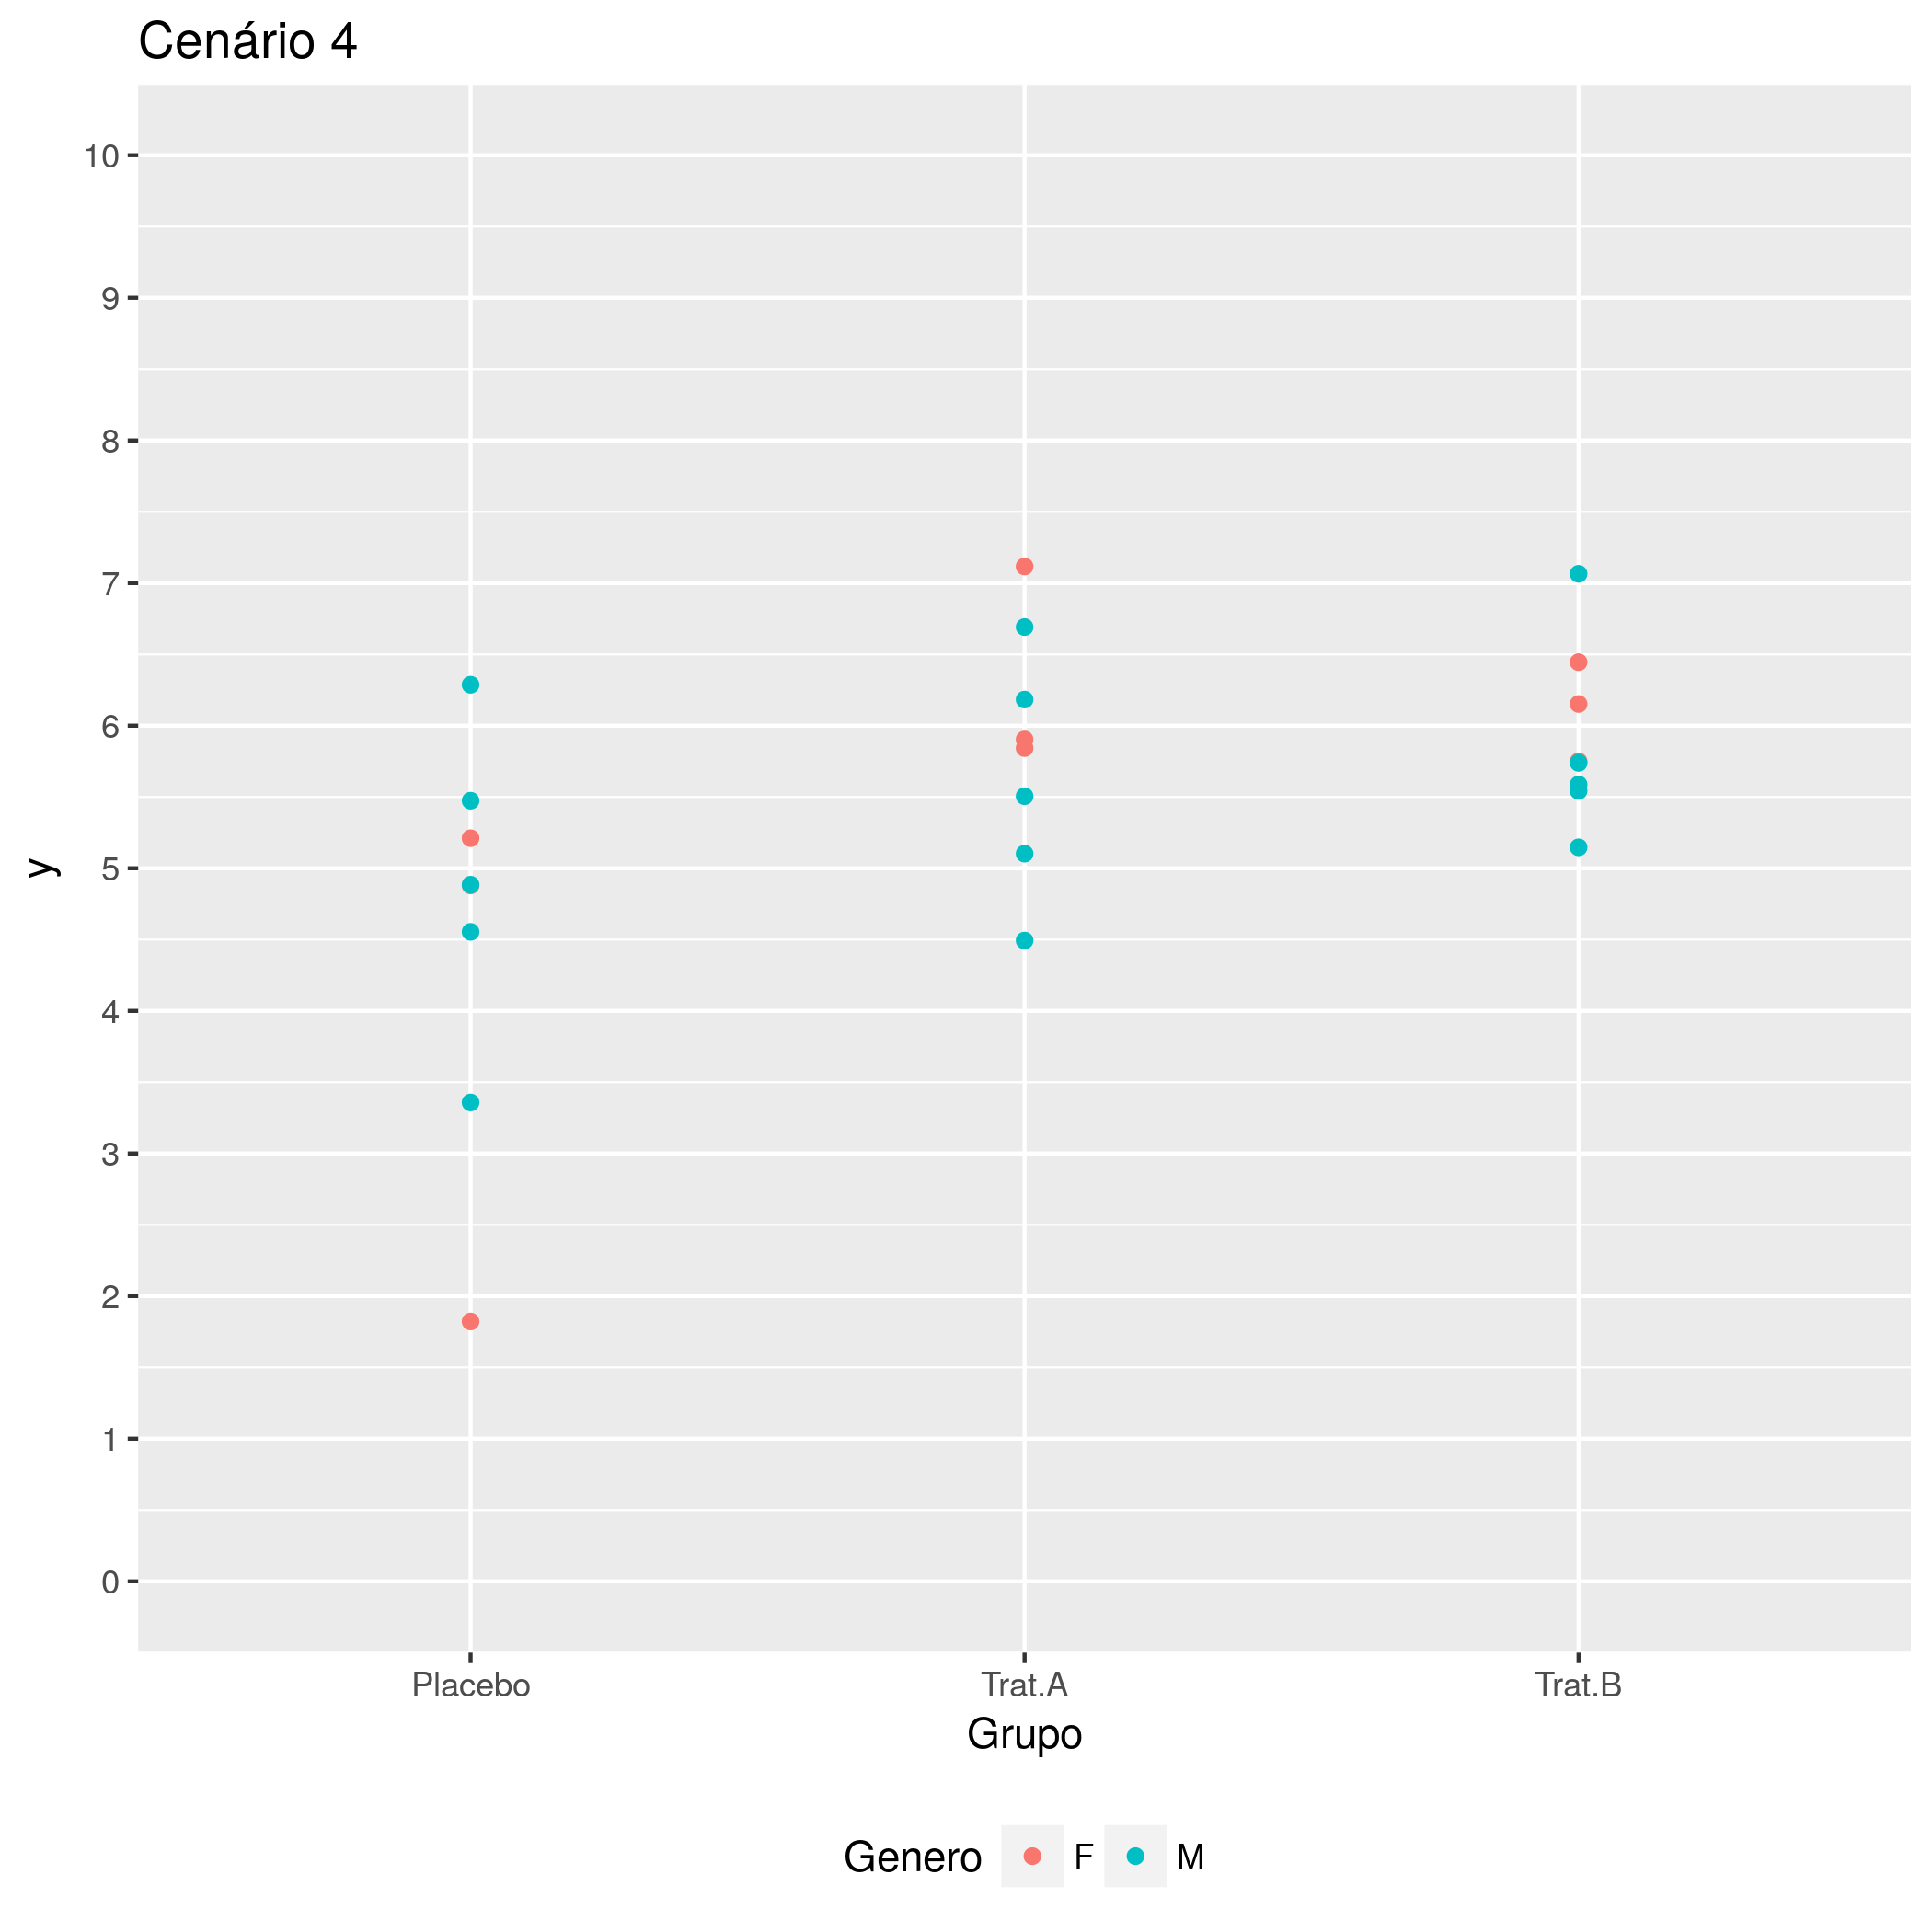
\includegraphics[height=.9\textheight]{Cap13-30/cenario22}
  \end{center}
\end{frame}

\begin{frame}
  \begin{center}
    Hora de testar seus conhecimentos
  \end{center}
\end{frame}

\section{Exercício}

\subsection{Exercício}

\begin{frame}[fragile]{Exercício}
  \begin{exampleblock}{Cenário 1 - ANOVA one-way}
    \tiny
\begin{verbatim}
            Df Sum Sq Mean Sq F value Pr(>F)
Grupo        2  4.124  2.0620   2.545  0.102
Residuals   21 17.018  0.8104
\end{verbatim}
    \begin{center}
      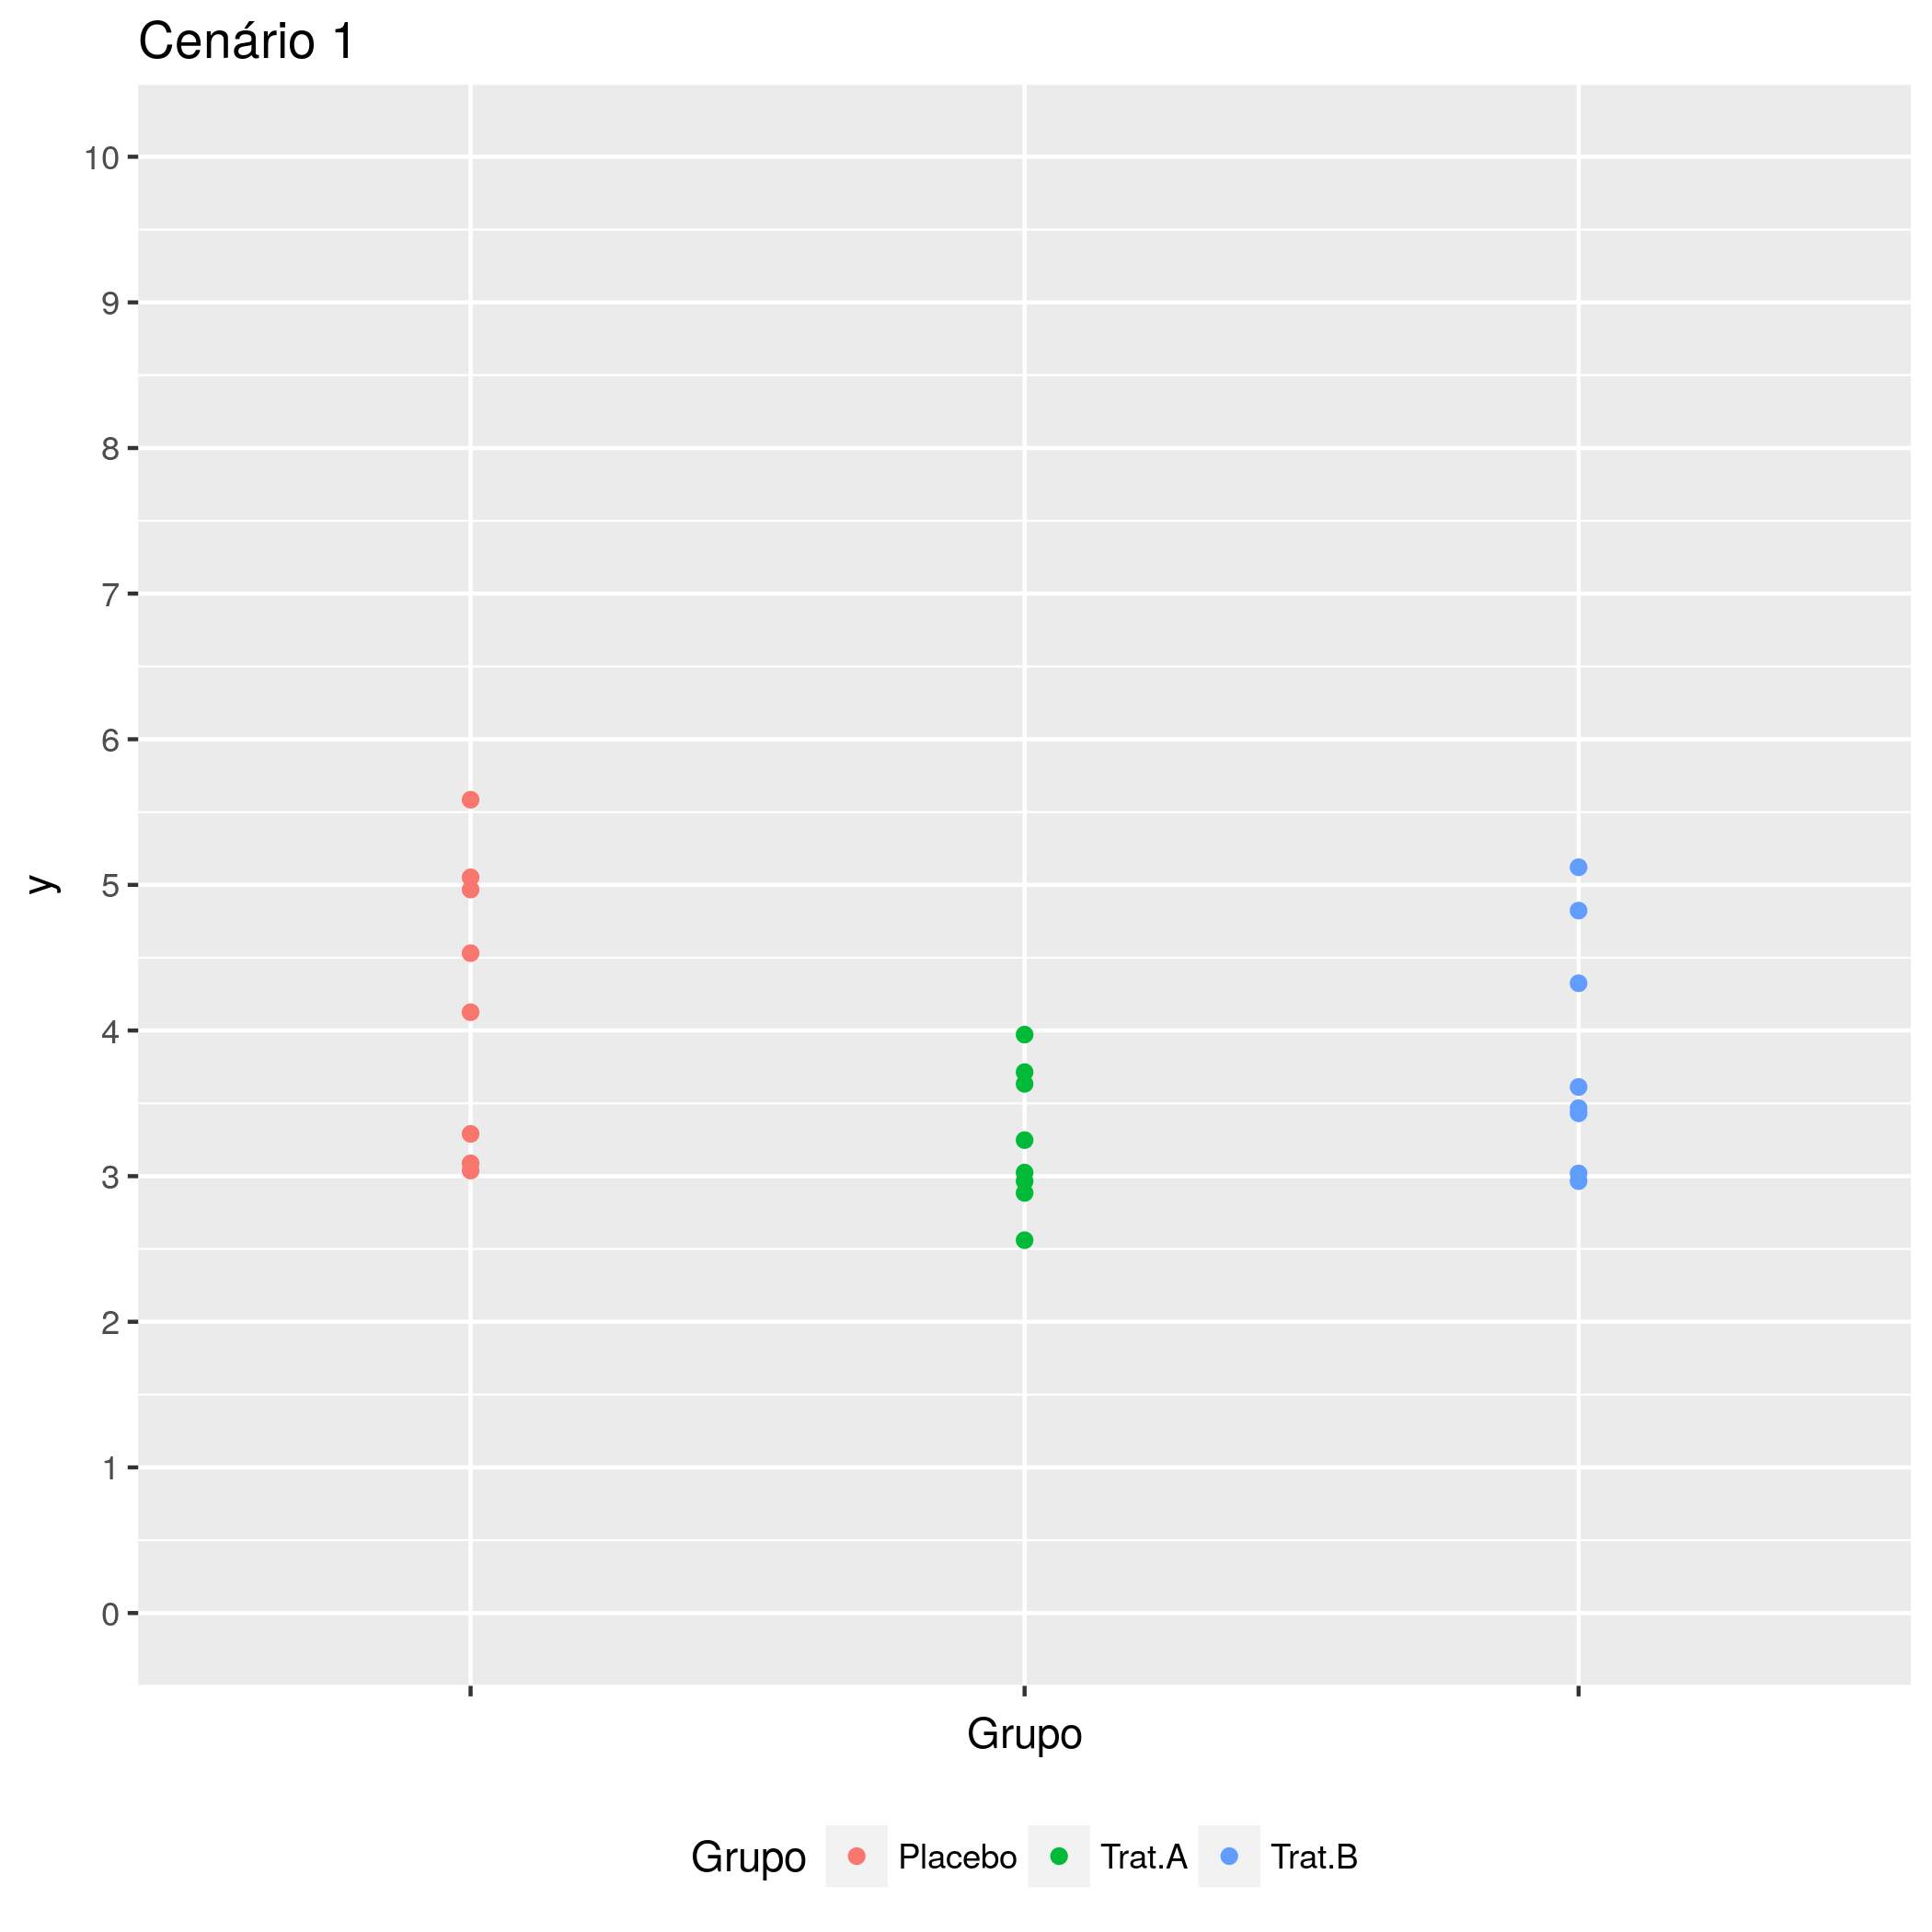
\includegraphics[height=.5\textheight]{Cap13-30/cenario1}
    \end{center}
  \end{exampleblock}
\end{frame}

\begin{frame}[fragile]{Exercício}
  \begin{exampleblock}{Cenário 3 - ANOVA two-way}
    \tiny
\begin{verbatim}
            Df Sum Sq Mean Sq F value Pr(>F)
Grupo        2  4.124  2.0620   2.426  0.114
Genero       1  0.020  0.0198   0.023  0.880
Residuals   20 16.998  0.8499
\end{verbatim}
    \begin{center}
      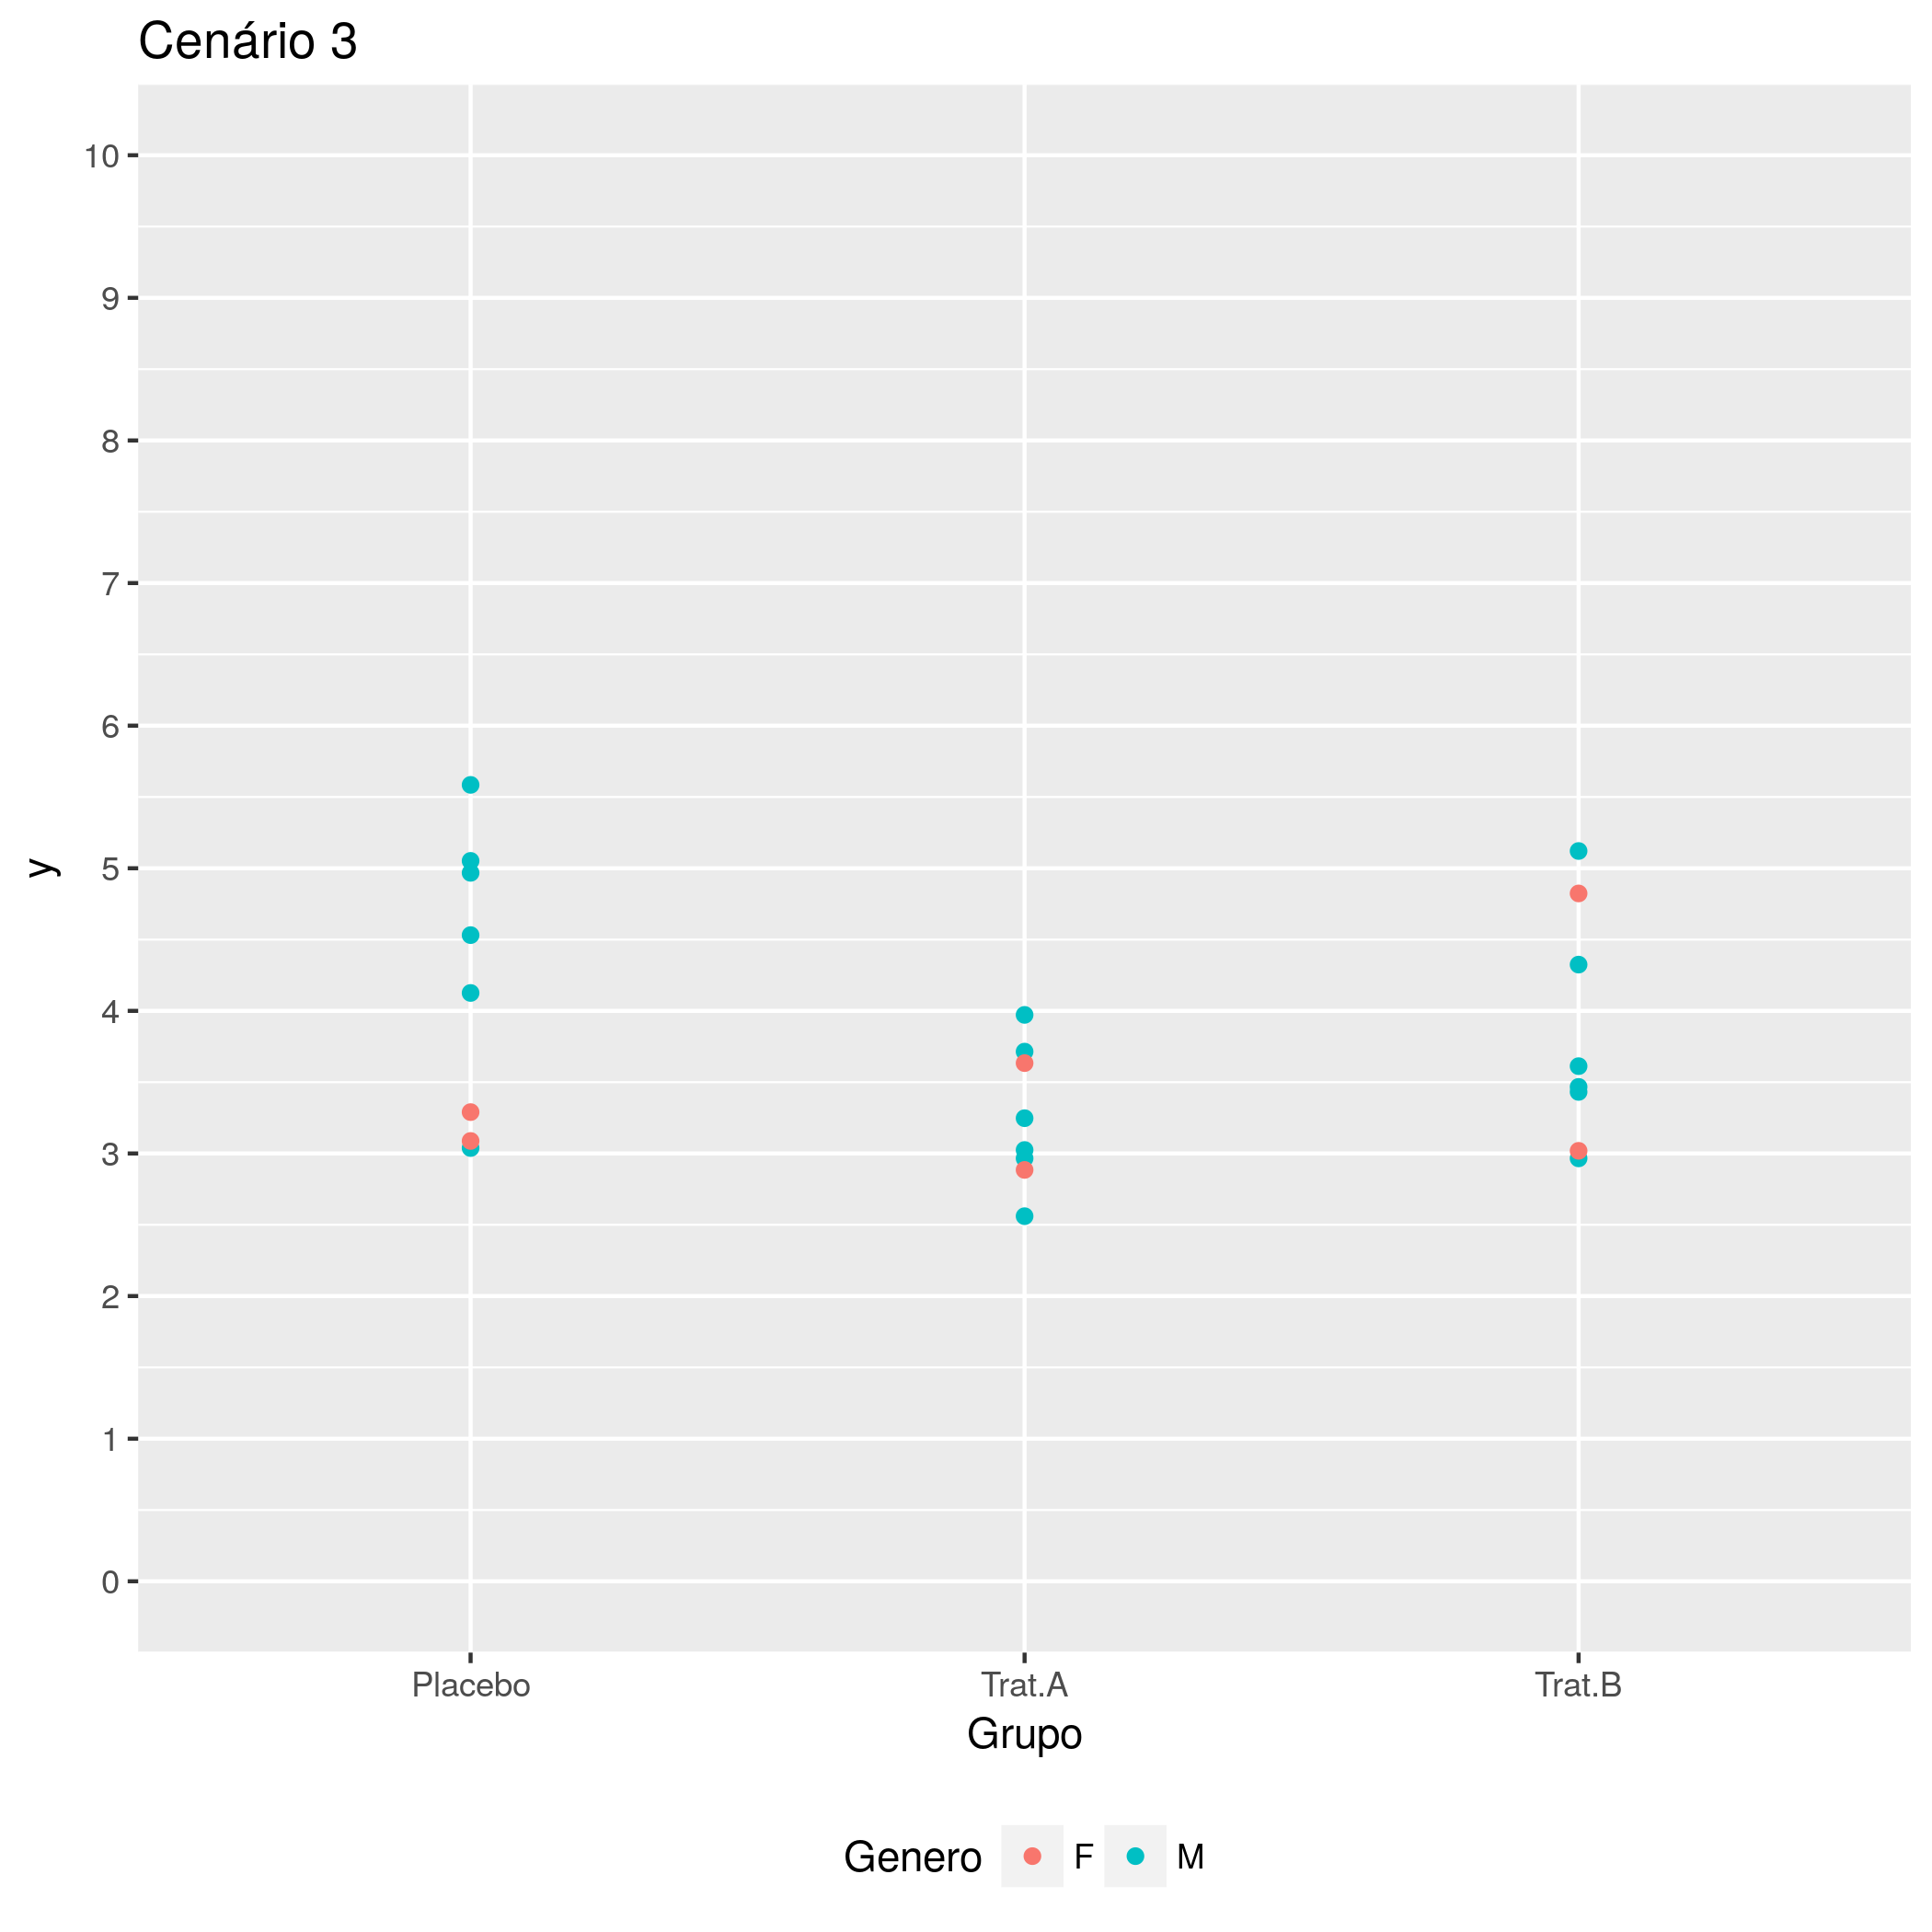
\includegraphics[height=.5\textheight]{Cap13-30/cenario12}
    \end{center}
  \end{exampleblock}
\end{frame}

\begin{frame}[fragile]{Exercício}
  \begin{exampleblock}{Cenário 2 - ANOVA one-way}
    \tiny
\begin{verbatim}
            Df Sum Sq Mean Sq F value   Pr(>F)
Grupo        2  32.99  16.496   25.04 2.75e-06 ***
Residuals   21  13.83   0.659
---
Signif. codes:  0 ‘***’ 0.001 ‘**’ 0.01 ‘*’ 0.05 ‘.’ 0.1 ‘ ’ 1
\end{verbatim}
    \begin{center}
      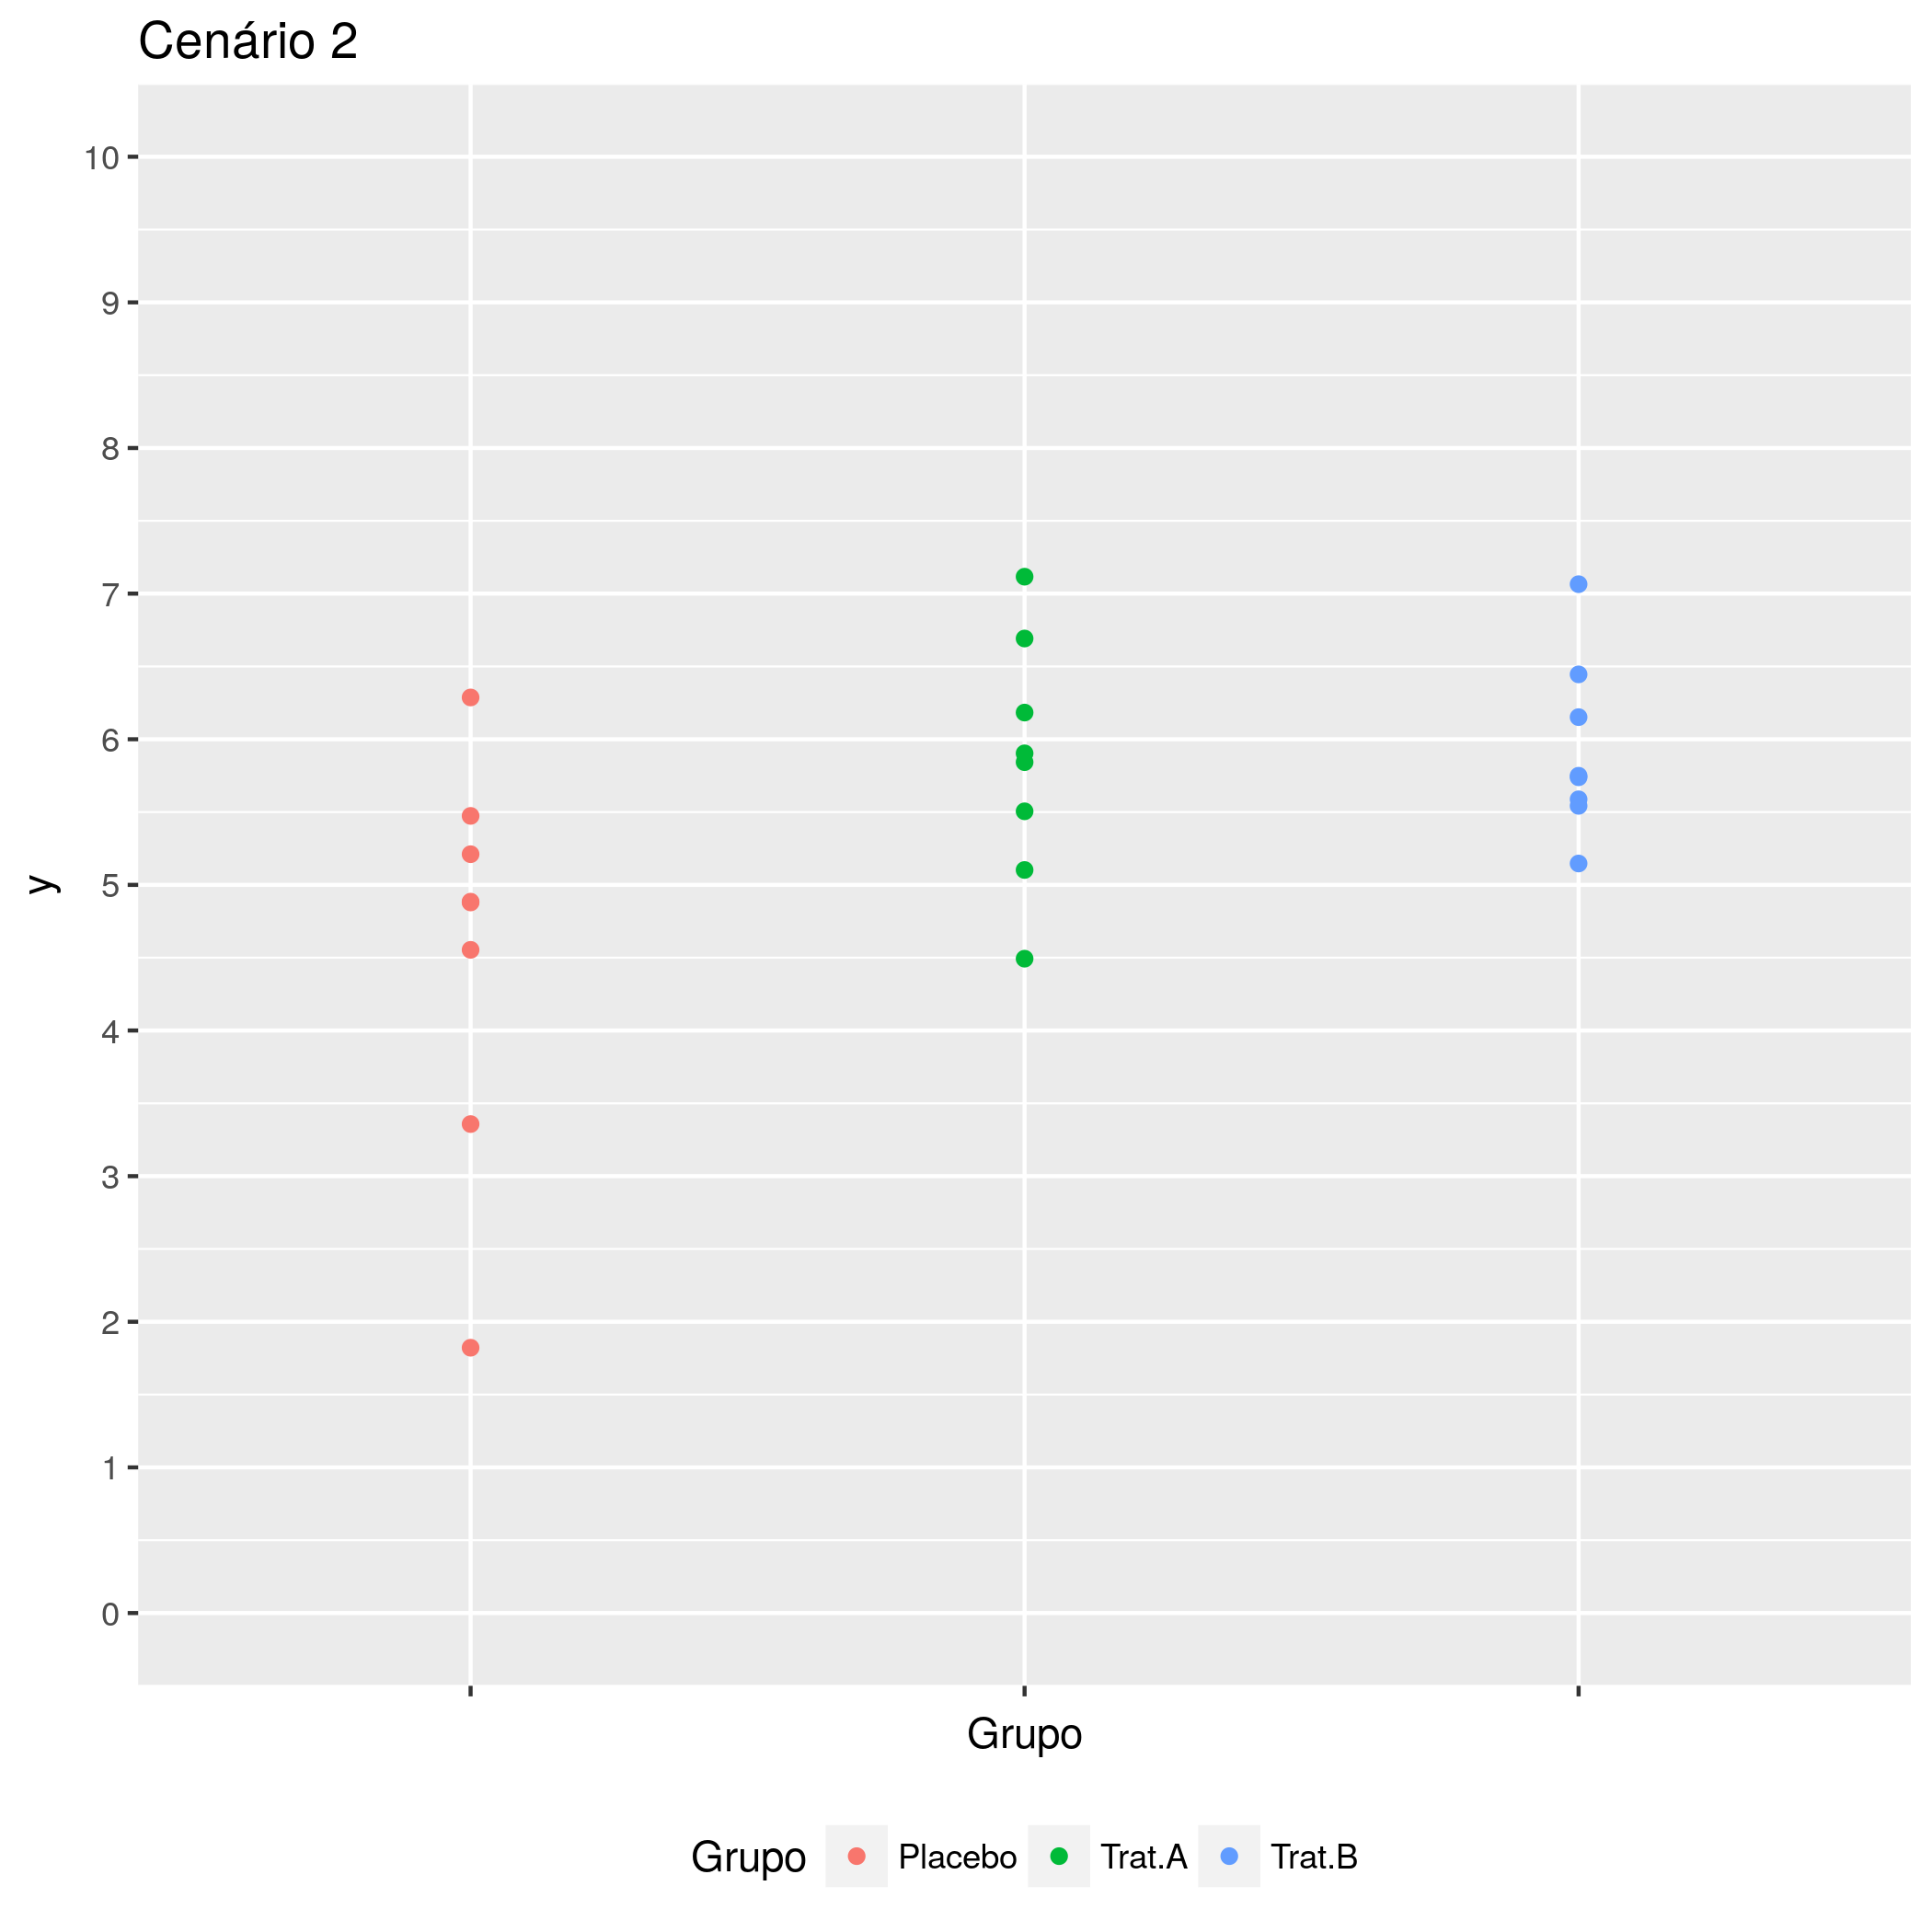
\includegraphics[height=.5\textheight]{Cap13-30/cenario2}
    \end{center}
  \end{exampleblock}
\end{frame}

\begin{frame}[fragile]{Exercício}
  \begin{exampleblock}{Cenário 2 - Tukey}
    \tiny
\begin{verbatim}
  Tukey multiple comparisons of means
    95% family-wise confidence level

Fit: aov(formula = y ~ Grupo, data = cenario2.long)

$Grupo
                     diff        lwr       upr     p adj
Trat.A-Placebo  2.8224313  1.7995273 3.8453353 0.0000021
Trat.B-Placebo  1.8711918  0.8482877 2.8940958 0.0004262
Trat.B-Trat.A  -0.9512395 -1.9741435 0.0716645 0.0713859
\end{verbatim}
  \end{exampleblock}
\end{frame}

\begin{frame}[fragile]{Exercício}
  \begin{exampleblock}{Cenário 4 - ANOVA two-way}
    \tiny
\begin{verbatim}
            Df Sum Sq Mean Sq F value   Pr(>F)
Grupo        2  32.99  16.496  24.760 3.88e-06 ***
Genero       1   0.51   0.509   0.764    0.393
Residuals   20  13.33   0.666
---
Signif. codes:  0 ‘***’ 0.001 ‘**’ 0.01 ‘*’ 0.05 ‘.’ 0.1 ‘ ’ 1
\end{verbatim}
    \begin{center}
      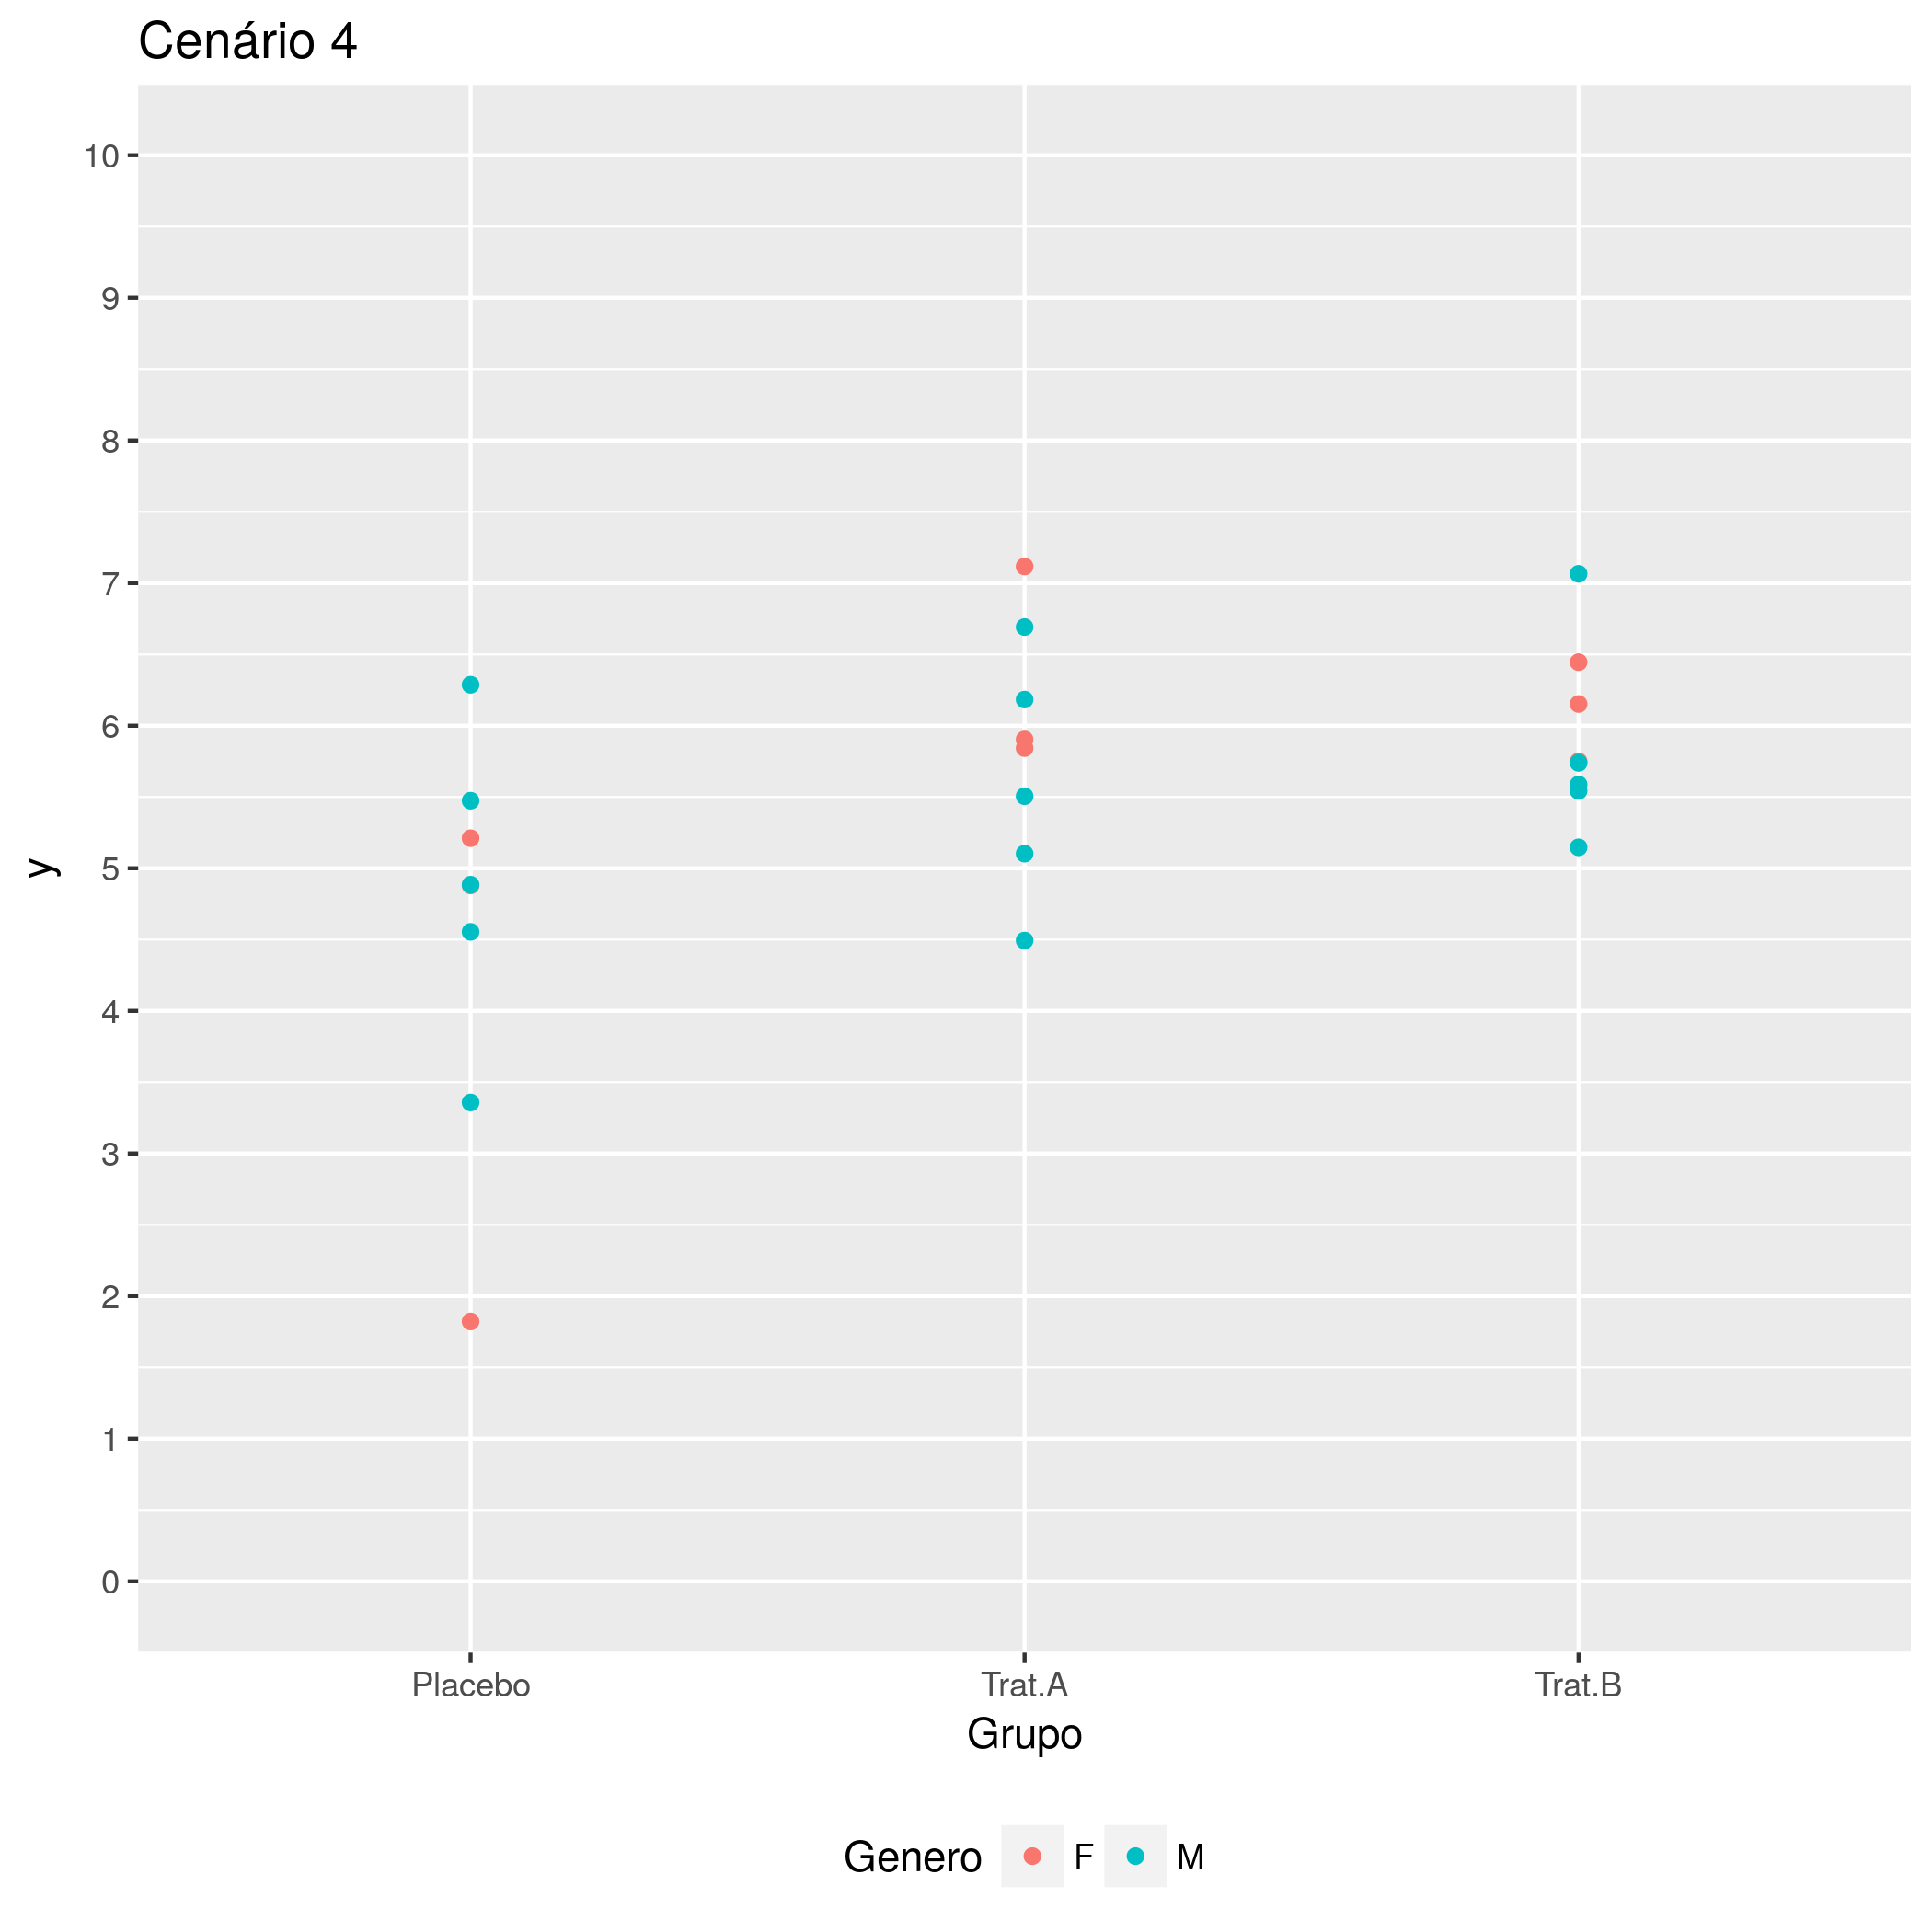
\includegraphics[height=.5\textheight]{Cap13-30/cenario22}
    \end{center}
  \end{exampleblock}
\end{frame}

\begin{frame}[fragile]{Exercício}
  \begin{exampleblock}{Cenário 4 - Tukey}
    \tiny
\begin{verbatim}
  Tukey multiple comparisons of means
    95% family-wise confidence level

Fit: aov(formula = y ~ Grupo + Genero, data = cenario2.long)

$Grupo
                     diff       lwr        upr     p adj
Trat.A-Placebo  2.8224313  1.789885 3.85497800 0.0000030
Trat.B-Placebo  1.8711918  0.838645 2.90373849 0.0005050
Trat.B-Trat.A  -0.9512395 -1.983786 0.08130722 0.0743628

$Genero
         diff        lwr      upr     p adj
M-F 0.3362835 -0.4663601 1.138927 0.3925159
\end{verbatim}
  \end{exampleblock}
\end{frame}

% \section{Encerramento}

% \subsection{Resumo}

% \begin{frame}{Resumo}
%   \begin{itemize}
%   \item
%   \end{itemize}
% \end{frame}

\section{Aprofundamento}

\subsection{Aprofundamento}

\begin{frame}{Aprofundamento}
  \begin{block}{Leitura obrigatória}
    \begin{itemize}
    \item Capítulo 13
    \item Capítulo 30
    \end{itemize}
  \end{block}
  \begin{block}{Exercícios selecionados}
    \small
    Capítulo 13, problema: 1
  \end{block}
  \begin{block}{Leitura recomendada}
    \small
    Não há.
  \end{block}
\end{frame}

\end{document}
